% !TeX root = proposal.tex
\chapter{Recommending Privacy Settings for Household IoT}\label{chapter:householdIoT}

In Chapter~\ref{chapter:generalIoT}, we have discussed recommending privacy preference for general IoT users. In this chapter, we present the work completed to date in the areas of designing for privacy for Household IoT. We expand and improve upon the previously-developed data-driven approach to design privacy-setting interfaces for users of household IoT devices. Moving the context to a more narrow environment shifts the focus of the privacy decision from the entity collecting information (which was the dominant parameter in our previous work) to a more contextual evaluation of the content or nature of the information ~\cite{nissenbaum_privacy_2004}. 

\section{Experimental Setup}\label{sec:exp_setup}
In Chapter~\ref{chapter:generalIoT}, we found that "where" does not have significant effect on disclosure decisions; also the usage environment of household IoT systems/devices are always in users' home. Moreover, the structure of users' houses are different from case to case, it would be too complicated if we define "where" to a more finer-granulated level, such as bedroom, kitchen, etc.,  Hence there there is no need to retain the parameter "where". ``Persistence" of tracking is more relevant in public IoT, where encounters are often ephemeral, hence persistent tracking is less common than in household IoT. ``Storage" and ``Action" allow us to explore secondary uses of the information; something we learned from the qualitative feedback in our previous study was a prominent concern among users.

Because of the above reasons, we conducted a new user study focusing on household IoT in particular, and further refine our approach to allow us to create more carefully tailored user interfaces. In this section, we first discuss the factorial procedure by which we developed 4608 highly specific IoT scenarios, as well as the questions we asked participants to evaluate these scenarios. We then describe the participant selection and experimental procedures used to collect over 13500 responses from 1133 participants.

\subsection{Contextual Scenarios}
The scenarios evaluated in our study are based on a full factorial combination of five different Parameters: Who, What, Purpose, Storage and Action. A total of $8(who)*12(what)*4(purpose)*4(storage)*3(action) = 4608$ scenarios were tested this way. 

The scenarios asked participants to imagine that they were owners and active users of the presented IoT devices, trying to decide whether to turn on or off certain functionalities and/or data sharing practices. To avoid endowment effects, the scenarios themselves made no indication as to whether the functionality was currently turned on or off (such endowment effects were instead introduced by manipulating the framing of the Decision question; see section \ref{sec:questions}). An example scenarios is: \emph{``Your smart TV (Who) uses a camera (What) to give you timely alerts (Purpose). The data is stored locally (Storage) and used to optimize the service (Action).''} This scenario may for example represent a situation where the smarthome system has detected (via camera) a delivery of package and then alerts the user (via the smart TV) about its arrival. In this particular scenario we note that the video data is stored locally to optimize service; this could mean that the smarthome system uses the video stream to (locally) train a package detection algorithm. Similarly, another example of scenario is: \emph{``Your Smart Assistant uses a microphone to detect your location in house. The data is stored on a remote server and shared with third parties to recommend you other services.''} Similarly, this scenario could represent a situation where the smarthome has detected (via microphone) it's user's location in the house and this information is shared to smart assistant. In the scenario, the data is stored on remote server and shared with third parties so that it can recommend additional services (like weather or local transportation) via third parties to the user.

The levels of all five parameters used in our experiment are shown in Table~\ref{tab:parameter2}. The parameters were highlighted in the scenario for easy identification, and upon hovering the mouse cursor over them each parameter would show a succinct description of the parameter. %\textcolor{blue}{Figure~\ref{fig:scenario} in the Appendix shows a screenshot of a scenario as shown to participants in the study.}
A thirteenth scenario regarding the interrelated control of various IoT devices (e.g. \emph{``You can use your smart TV to control your smart refrigerator''}) was also asked, but our current analysis focuses on the information-sharing scenarios only.

\subsection{Scenario Evaluation Questions}
\label{sec:questions}
The first question participants were asked about each scenario was whether they would enable or disable the particular feature mentioned in scenario (Decision). Subsequently, they were asked about their attitudes regarding the scenario in terms of their perceived Risk, Appropriateness, Comfort, Expectedness and Usefulness regarding the presented scenario (e.g., \emph{``How appropriate do you think this scenario is?''}). These questions were answered on a 7-point scale (e.g., \emph{``very inappropriate''} to \emph{``very appropriate''}). In every 4th scenario, the Risk and Usefulness questions were followed by an open question asking the participants to describe the potential Risk and Usefulness of the scenario. We asked these question mainly to encourage participants to carefully evaluate the scenarios.%A screenshot of the questions asked about each scenario is depicted in Figure~\ref{fig:scenario} in the Appendix.

%In addition to the twelve scenarios, the participants were also presented with a 13th scenario. This scenario was focused on giving the participants an ability to control for collection of information by devices. This was done by changing the for \emph{Who} and \emph{What} parameters. However, the rest of the parameters were kept same while forming the scenario. 
The framing and default of the Decision question were manipulated between-subjects at three levels each: positive framing (``Would you enable this feature?'', options: Yes/No), negative framing (``Would you disable this feature?'', options: Yes/No) or neutral framing (``What would you do with this feature?'', options: Enable/Disable); combined with a positive default (enabled by default), negative default (disabled by default), or no default (forced choice).


\begin{table}
	\centering
	\caption{Parameters used to construct the information-sharing scenarios. The ``codes'' are used as abbreviations in graphs and figures throughout the paper and the Appendix.}
	\label{tab:parameter2}
	\begin{tabular} {l|l|l}
		\hline
		\textbf{Parameter} & \textbf{Levels} & \textbf{Code} 	 \\ \hline
		Who:  & 1. Home Security System & SS\\ 		
		\emph{Your Smart...}	& 2. Refrigerator & RE							 \\
		& 3. HVAC System							& HV	 \\
		& 4. Washing Machine						& WM		 \\
		& 5. Lighting System						& SL	 \\
		& 6. Assistant 							 &SA\\
		& 7. TV 							 &TV\\
		& 8. Alarm Clock							&SC \\ \hline
		What:  & 1. Home Security System & CSE\\
		\emph{...uses information } & 2. Refrigerator &CRE							 \\
		\emph{collected by your...} & 3. HVAC System &CHV								 \\
		& 4. Washing Machine						& CWA		 \\
		& 5. Lighting System						&CLI	 \\
		& 6. Assistant 							 & CAS\\
		& 7. TV 							 & CTV\\
		& 8. Alarm							 & CAL\\
		& 9. uses a location sensor			&CLO	\\	
		& 10. uses a camera				& CCA\\	
		& 11. uses a microphone			& CMP				\\	
		& 12. connects to your smart phone/watch &CSW				\\\hline
		Purpose : & 1. detect whether you are home & PH		\\
		\emph{...to...} & 2. detect your location in house &LH		\\				
		& 3. automate its operations &AO\\
		& 4. give you timely alerts & TA\\ \hline
		%Who (Control):& 1. Assistant \\
		%\emph{"You can use your} & 2. TV							 \\
		%\emph{Smart...} & 3. Alarm Clock								 \\
		%& 4. Phone/Watch								 \\\hline
		%What (Control): & 1. Home Security System \\
		%\emph{...to control your...} & 2. Refrigerator							 \\
		%& 3. HVAC System								 \\
		%& 4. Washing Machine								 \\
		%& 5. Lighting System							 \\
		%& 6. Assistant 							 \\
		%& 7. TV 							 \\
		%& 8. Alarm Clock							 \\ \hline
		Storage:  & 1. locally	& L\\
		\emph{The data is stored...} & 2. on remote server & R						\\
		& 3. on a remote server and & T\\
		& shared with third parties &\\\hline
		Action: & 1. optimize the service & O \\
		\emph{...and used to... } & 2. give insight into your behavior& I \\
		& 3. recommend you other services & R\\
		& 4. [None] & N\\ \hline
	\end{tabular}
\end{table}

\subsection{Participants and Procedures}
To collect our dataset, 1133 adult U.S.-based participants (53.53\% Female, 45.75\% Male, 8 participants did not disclose) were recruited through Amazon Mechanical Turk. Participation was restricted to Mechanical Turk workers with a high reputation (at least 50 completed tasks completed with an average accuracy greater than 95\%). Participants were paid \$2.00 upon successful completion of the study. The participants were warned about not getting paid in case they failed attention checks.

The study participants represented a wide range of ages, with 9 participants less than 20 years old, 130 aged 20-25, 273 aged 25-30, 418 aged 30-40, 175 aged 40-50, 80 aged 50-60, and 43 participants over 60 years old (5 participants did not disclose their age). This significant increase in participants over the Lee and Kobsa~\cite{lee2016understanding} dataset is commensurate with our expectation of more complex privacy decision behaviors in household IoT compared to public IoT.

Each participant was first shown a video with a brief introduction to various smart home devices, which also mentioned various ways in which the different appliances would cooperate and communicate within a home. After the video, participants were asked to answer three attention check questions. If they got any of these questions wrong, they would be asked to read the transcript of the video and re-answer the questions.

After the introduction video, each participant was presented with 12 information-sharing scenarios (and a 13th control scenario, not considered in this paper). These scenarios were selected from the available 4608 scenarios using fractional factorial design\footnote{The scenario assignment scheme is available at \url{https://www.usabart.nl/scenarios.csv}} that balances the within- and between-subjects assignment of each parameter's main effect, and creates a uniform exposure for each participant to the various parameters (i.e., to avoid ``runs'' of near-similar scenarios). Participants were asked to carefully read the scenario and then answer all questions about it. Two of the 13 scenarios had an additional attention check question (e.g., ``Please answer this question with Completely Agree'', and there was an additional attention check question asking participants about the remaining time to finish the study (which was displayed right there on the same page. Participants rushing through the experiment and/or repeatedly failing the attention check questions were removed from the dataset.
%
%\section{Inspecting Users' Decisions}\label{sec:inspect}
%In this section we explain the different regression analyses performed on the dataset to understand how different scenario parameters affected the decisions made by participants. We begin by explaining the effects of scenario parameters on participants' decision to enable or disable the feature mentioned in the scenario. Similar to Bahirat et. al., we also present the results of the mediation analysis, which are on the lines of attitude-behavior models~\cite{bahiratiui2018,ajzen1977attitude}. As shown in Figure~\ref{fig:mediation_test}, we test whether participants' attitudes mediate the effects of the scenario parameters on their decisions. This mediation analysis involves the following tests:
%
%\textbf{Test 1}: The effect of parameters (Who, What, Purpose, Storage, Action) on attitudes (Risk, Comfort, Appropriateness, Expectedness and Usefulness).
%
%\textbf{Test 2}: The effect of attitudes on decision.
%
%\textbf{Test 3}: The effect of both parameters \emph{and} attitudes on decision.
%
%If, tests 1 and 2 are significant and test 3 reveals a drastic reduction in the conditional direct effect of parameters, then we can say that the effects of scenario parameters on participant's decision are mediated by their attitudes~\cite{bahiratiui2018}.
%
%
%\begin{figure}
%	\centering
%	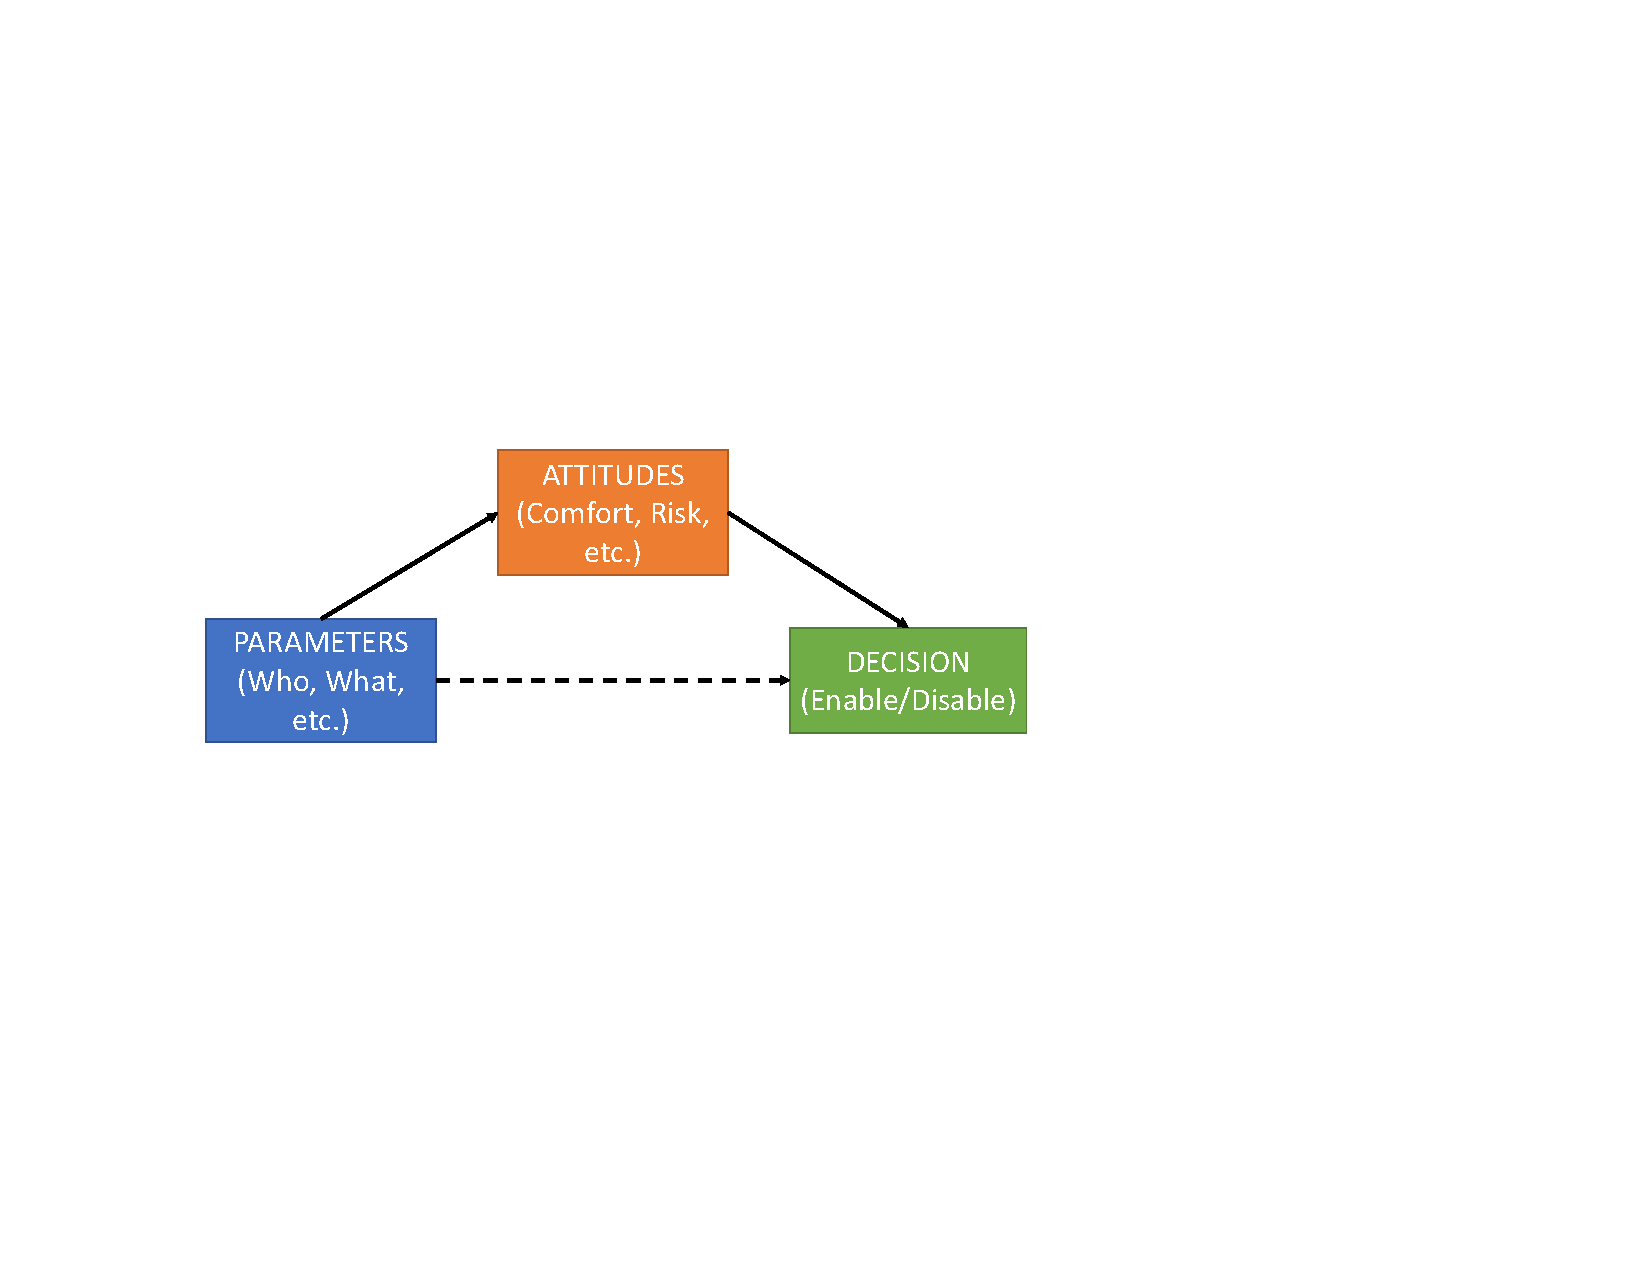
\includegraphics[width=0.75\textwidth]{figures/mediation_test.pdf}
%	\caption{Different tests conducted for mediation analysis}
%	\label{fig:mediation_test}
%\end{figure}
%
%
%Finally, we present a post-hoc analysis of differences between individual levels of the parameters on attitudes and decision.
%
%\subsection{Effect of scenario parameters on decision}
%To understand the effect of the scenario parameters on participants' allow/reject decision, we developed a \emph{generalized linear mixed effects regression} (\emph{glmer}) with a random intercept (to account for repeated measures on the same participant) and a logit link function (to account for the fact that the outcome variable is binary). We used a forward stepwise approach, where we added the strongest remaining parameter into the model into the model at each step and then comparing it using ANOVA tests against the previous model. If new parameter makes a significant improvement to the previous model, it has a significant overall effect on the outcome variable. Once all significant main effects are added to the model, two-way interaction effects are tested one by one. 
%
%Table~\ref{tab:para_decision} shows the effects of the parameters on the allow/reject decision. All parameters had a significant effect. Particularly, \textbf{Storage} had the strongest effect on participants' decisions, followed by \textbf{What}, \textbf{Who} and \textbf{Purpose} (all similar) and finally \textbf{Action}.
%
%Moreover, we find many significant interaction effects, but some of them are not substantial compared to the main effects\footnote{Very small but still significant interaction effects are a common occurrence in the analysis of large datasets.}. Substantial two-way interaction effects were observed between \textbf{Who}, \textbf{What} and \textbf{Purpose}. It should be noted that the interactions are added separately, not accumulatively. This reduces overfitting and multicollinearity.
%
%\begin{table}
%	\centering
%	\caption{Effect of scenario parameters on decision}
%	\label{tab:para_decision}
%	\begin{tabular}{ l | r | r | r }
%		\hline
%		Model &	$\chi^2$ & $df$ & $p$-value 	\\ \hline
%		$decision\sim(1 | sid)$ &		  	&	    &				\\
%		+storage &					1487.76	& 	  2 & 		$<$ .0001 	\\
%		+purpose &					206.97 &		  11 &		$<$ .0001 	\\
%		+what &				202.48 & 	  3 & 		  	$<$ .0001	\\
%		+who &			195.91 &		  7 & 		$<$ .0001 	\\
%		+action &			77.20 &		  3 & 		$<$ .0001\\\hline
%		\emph{Interactions}&			 &		  & \\\hline
%		+what:who &			138.03 &		  77 & 		$<$ .0001\\
%		+who:purpose &			87.92 &		  21 & 		$<$ .0001\\
%		+what:purpose &			68.30 &		  33 & 		.0002\\
%		\hline
%	\end{tabular}
%\end{table}
%
%\subsection{Effect of scenario parameters on attitudes}
%Test 1 of the mediation model is a test of the effect of the scenario parameters on participants' attitudes. For this we developed a separate \emph{linear mixed effects regression model} (\emph{lmer}) model with a random intercept (to account for repeated measures on the same participant) for each dependent variable (Risk, Comfort, Appropriateness, Expectedness and Usefulness), using the scenario parameters as independent variables. As in the previous section, we took a forward stepwise approach.
%
%Tables~\ref{tab:para_approp}-\ref{tab:para_exp} show the effects of the parameters on the different attitudes. All parameters had a significant effect on all attitudes. Substantial two-way interaction effects were again observed between \textbf{Who}, \textbf{What} and \textbf{Purpose}. Again, the interactions are added separately, not accumulatively.
%
%\begin{table}
%	\centering
%	\caption{Effect of scenario parameters on appropriateness}
%	\label{tab:para_approp}
%	\begin{tabular}{ l | r | r | r }
%		\hline
%		Model &	$df$ & $Chi. Sq.$ & $p$-value 	\\ \hline
%		$appropriateness\sim(1 | sid)$ &	3	  	&	    &				\\
%		+storage &					5	& 	  2346.19 & 		$<$ .0001 	\\
%		+what &					16 &		  398.63 &		$<$ .0001 	\\
%		+purpose &				19 & 	  359.98 & 		  	$<$ .0001	\\
%		+who &			26 &		  179.09 & 		$<$ .0001 	\\
%		+action &			29 &		  91.05& 		$<$ .0001\\\hline
%		\emph{Interactions}&			 &		  & \\\hline
%		+what:who &			106 &		  167.01 & 		$<$ .0001\\
%		+who:purpose &			50 &		  113.73 & 		$<$ .0001\\
%		+what:purpose &			62 &		  55.67 & 		.0081\\
%		\hline
%	\end{tabular}
%\end{table}
%
%\begin{table}
%	\centering
%	\caption{Effect of scenario parameters on comfort}
%	\label{tab:para_comfort}
%	\begin{tabular}{ l | r | r | r }
%		\hline
%		Model &	$df$ & $Chi. Sq.$ & $p$-value 	\\ \hline
%		$comfort\sim(1 | sid)$ &	3	  	&	    &				\\
%		+storage &					5	& 	  2822.57 & 		$<$ .0001 	\\
%		+what &					16 &		  391.10 &		$<$ .0001 	\\
%		+purpose &				19 & 	  381.69 & 		  	$<$ .0001	\\
%		+action &			22 &		  113.68 & 		$<$ .0001 	\\
%		+who &			29 &		  90.57& 		$<$ .0001\\\hline
%		\emph{Interactions}&			 &		  & \\\hline
%		+what:who &			106 &		  132.86 & 		$<$ .0001\\
%		+who:purpose &			50 &		  89.20 & 		$<$ .0001\\
%		+what:purpose &			62 &		  58.24 & 		 .0043\\
%		\hline
%	\end{tabular}
%\end{table}
%
%\begin{table}
%	\centering
%	\caption{Effect of scenario parameters on risk}
%	\label{tab:para_risk}
%	\begin{tabular}{ l | r | r | r }
%		\hline
%		Model &	$df$ & $Chi. Sq.$ & $p$-value 	\\ \hline
%		$risk\sim(1 | sid)$ &	3	  	&	    &				\\
%		+storage &					5	& 	  47240.72 & 		$<$ .0001 	\\
%		+purpose &					16 &		  421.08 &		$<$ .0001	\\
%		+action &				19 & 	  355.65 & 		  	$<$ .0001	\\
%		+who &			26 &		  81.35 & 		 $<$ .0001 	\\
%		+what &			29 &		  70.64 & 		 $<$ .0001\\\hline
%		\emph{Interactions}&			 &		  & \\\hline
%		+what:who &			106 &		  77.14 & 		 0.0017\\
%		+who:purpose &			50 &		  19.91 & 		$<$ .0001\\
%		+what:purpose &			62 &		  37.19 & 		0.0352\\
%		\hline
%	\end{tabular}
%\end{table}
%
%\begin{table}
%	\centering
%	\caption{Effect of scenario parameters on usefulness}
%	\label{tab:para_use}
%	\begin{tabular}{ l | r | r | r }
%		\hline
%		Model &	$df$ & $Chi. Sq.$ & $p$-value 	\\ \hline
%		$usefulness\sim(1 | sid)$ &	3	  	&	    &				\\
%		+what &					5	& 	  939.91 & 		$<$.0001 	\\
%		+storage &					12 &		  457.36 &		$<$.0001	\\
%		+purpose &				23 & 	  401.18 & 		  	$<$.0001	\\
%		+action &			26 &		  328.88 & 		 $<$.0001 	\\
%		+who &			29 &		  117.57& 		 $<$.0001\\\hline
%		\emph{Interactions}&			 &		  & \\\hline
%		+what:who &			106 &		 214.48 & 		 $<$.0001\\
%		+who:purpose &			50 &		  184.48 & 		$<$.0001\\
%		+what:purpose &			62 &		  85.39 & 		$<$.0001\\
%		\hline
%	\end{tabular}
%\end{table}
%
%\begin{table}
%	\centering
%	\caption{Effect of scenario parameters on expectedness}
%	\label{tab:para_exp}
%	\begin{tabular}{ l | r | r | r }
%		\hline
%		Model &	$df$ & $Chi. Sq.$ & $p$-value 	\\ \hline
%		$expectedness\sim(1 | sid)$ &	3	  	&	    &				\\
%		+storage &					5	& 	  841.24 & 		$<$ .0001 	\\
%		+who &					16 &		  425.92 &		$<$ .0001 	\\
%		+what &				19 & 	  422.31 & 		  	$<$ .0001	\\
%		+purpose &			22 &		  231.98 & 		$<$ .0001 	\\
%		+action &			29 &		  29.45& 		$<$ .0001\\\hline
%		\emph{Interactions}&			 &		  & \\\hline
%		+what:who &			106 &		  262.80 & 		$<$ .0001\\
%		+who:purpose &			50 &		  138.73 & 		$<$ .0001\\
%		+what:purpose &			62 &		  84.89 & 		$<$ .0001\\
%		\hline
%	\end{tabular}
%\end{table}
%
%\subsection{Effect of attitudes on decision}
%Test 2 of the mediation model is a test of the effect of participants' attitudes on their allow/reject decision. We perform this test by creating a \emph{glmer} model with a random intercept and a logit link function. Using a forward stepwise approach, we find that all attitudes except \textbf{Expectedness} have a significant effect on decision (see the top part of Table~\ref{tab:att_decision}). Specific effects are as follows:
%\begin{itemize}
%	\item Each 1-point increase in \textbf{Comfort} (measured on a 7-point scale) results in a 2.30-fold increase in the odds that the participant will allow the scenario ($p < 0.001$). 
%	\item Each 1-point increase in \textbf{Usefulness} results in a 2.09-fold increase in the odds that the participant will allow the scenario ($p < 0.001$).
%	\item Each 1-point increase in \textbf{Appropriateness} results in a 44\% increase in the odds that the participant will allow the scenario ($p < 0.001$).
%	\item Each 1-point increase in \textbf{Risk} results in a 14\% decrease in the odds that the participant will allow the scenario ($p < 0.001$).
%	\item \textbf{Expectedness} had no signficant influence on the participant's decision (p = 0.201).
%\end{itemize}
%
%
%\begin{table}
%	\centering
%	\caption{Effect of attitudes on decision; conditional effects of parameters are added subsequently}
%	\label{tab:att_decision}
%	\begin{tabular}{ l | r | r | r }
%		\hline
%		Model &	$\chi^2$ & $df$ & $p$-value 	\\ \hline
%		$decision\sim(1 | sid)$ &		  	&	    &				\\
%		+Comfort &					7934.72	& 	  1 & 		$<$ .0001 	\\
%		+Usefulness &					1249.51 &		  1 &		$<$ .0001 	\\
%		+Appropriateness &				149.15 & 	  1 & 		  	$<$ .0001	\\
%		+Risk  &			10.90 &		  1 & 		 .0009 	\\
%		+Expectedness &			1.62 &		  1 & 		 .201\\\hline
%		\emph{Adding Scenario Parameters}&			 &		  & \\\hline
%		+action &			0.332 &		  3 & 		 0.953\\
%		+what &			13.871 &		  11 & 		0.2401\\
%		+purpose &			3.60 &		  3 & 		0.3069\\
%		+storage &			14.57 &		  2 & 		0.0006\\
%		+who &			24.53 &		  7 & 		0.0009\\
%		\hline
%	\end{tabular}
%\end{table}
%
%\textcolor{blue}{The strongly significant relationship between attitudes and behavior is interesting in light of the ``privacy paradox''~\cite{norberg07}, an attitude-behavior gap that has been studied extensively by privacy researchers. Arguably, the privacy paradox is an artifact of the fact that \emph{general} privacy concerns (which are commonly high) do not match \emph{specific} behaviors (which subsequently ignore these general concerns). Since in our study attitudes and behaviors are measured at the same contextual level, their relationship is much stronger than in other studies. This may explain why we do not find an attitude-behavior gap.}
%
%
%\subsection{Mediation analysis}
%With tests 1 and 2 of our mediation analysis confirmed, we conduct test 3 by adding the scenario parameters to the \emph{glmer} of participants' decisions on their attitudes. The bottom half of Table~\ref{tab:att_decision} shows these conditional effects of the significant scenario parameters on participants' allow/reject decision, controlling for their attitudes. \textbf{Action}, \textbf{What} and \textbf{Purpose} are no longer significant in this model, suggesting that these effects are \emph{fully mediated} by participants' attitudes. \textbf{Storage} and \textbf{Who} are still significant, but their conditional effects are smaller than their marginal effects on decision (without controlling for attitude, see Table~\ref{tab:para_decision}). Their $chi^2$s are reduced drastically by 98\% and 87\%, respectively. Overall, there was a substantial mediation effect. Figure~\ref{fig:mediation_model} shows the final model mediation model.
%
%\begin{figure}
%	\centering
%	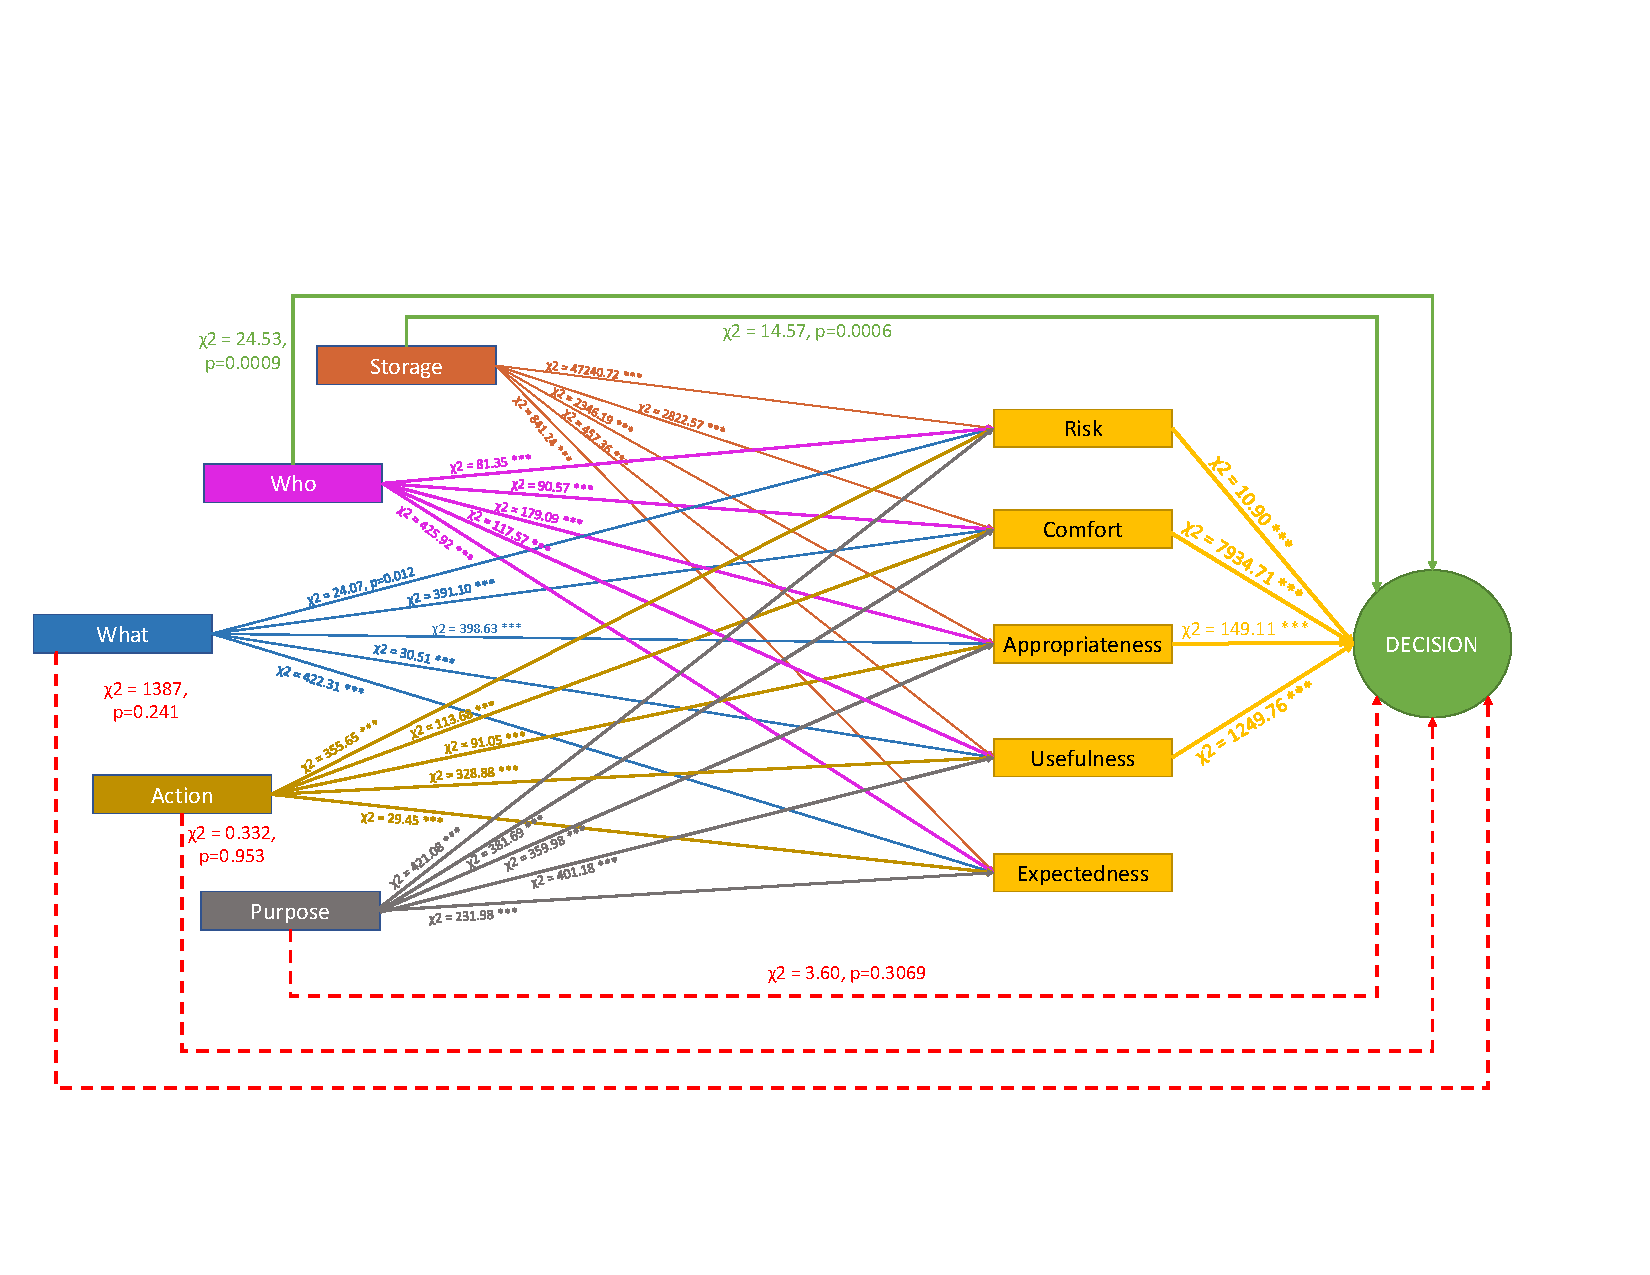
\includegraphics[width=0.95\textwidth]{figures/mediation.pdf}
%	\caption{Final mediation model.}
%	\label{fig:mediation_model}
%\end{figure}
%
%
%\subsection{Post-hoc Results}
%To understand the effects of different values of each parameter on participants' various attitudes and their allow/reject decision, we conducted \textcolor{blue}{post-hoc tests using Tukey's method to adjust $p$-values to account for familywise error.} This subsection highlights the key insights from these tests. For an overview of the differences between parameter values, the reader is invited to visually inspect them by referring to Figures~\ref{fig:storage_post}-\ref{fig:what_post} in the Appendix.
%
%\textbf{Storage}: Participants perceive more risk ($d$ range $= [0.568, 1.707]$, all $p$s $< .001$), are less comfortable ($d$ range $= [0.538, 1.741]$, all $p$s $< .001$) and find it inappropriate ($d$ range  $=  [0.436, 1.550]$, all $p$s $< .001$) when their information is shared to `third parties' or `stored on a remote server' as compared to when it is stored `locally'. Participants also found it less useful to share their information with third parties as compared to storing it locally or on a remote server ($d$ range $= [0.28, 1.02]$,  $p < .001$). Interestingly, participants expected it less that the information is stored locally rather than stored on remote server or shared to third parties ($d$ range $= [0.212, 0.894]$, all $p$s $< .001$). Finally, the odds of enabling a feature when information is stored locally were 1.96 times higher than when information is stored on a remote server ($p < .001$) and 8.36 times higher than when information is shared with third parties ($p < .001$).
%
%\textbf{Action}: Participants were less comfortable ($d$ range $= [0.158, 0.348]$, all $p$s $< .001$) and found it more risky ($d$ range $= [0.145, 0.262]$, all $p$s $< .001$) when their information is used to give them recommendations instead of optimizing services or giving them insight into their behavior. Sharing information was also found less useful ($d = 0.293$, $p < .001$) and less appropriate ($d = 0.256$, $p < .001$) for recommendation purposes as opposed to when the scenario did not specify any purpose. Participants also expected it less ($d = 0.123$, $p = .0021$) when their information was being shared for recommendation purposes as opposed to when the scenario did not specify any purpose. Finally, the odds of enabling a feature for recommendation purposes were 1.53 times lower as opposed to when the scenario did not specify any purpose ($p < .001$). Additionally, the odds of enabling a feature for optimization purposes were 1.65 times higher than for recommendation purposes ($p < .001$) and 1.26 times higher than for giving behavioral insights ($p < .001$). 
%
%\textbf{Purpose}: Participants found it inappropriate ($d$ range $= [0.343, 0.411]$, all $p$s $< .001$) when information is collected for the purpose of detecting their presence in the house as compared to the purposes of automating operations or giving timely alerts, and it was even more inappropriate to collect information for the purpose of detecting their location in the house ($d$ range $= [0.163, 0.574]$, all $p$s $< .001$). Participants also found it more risky when information is used for location detection as compared to presence detection ($d = 0.598$, $p < .001$), but they found it less risky to share information for the purpose of giving timely alerts or for automating operations ($d$ range  $= [0.550, 0.601]$, $p$ range $= [0.002, 0.004]$). Participants also found it more useful when information is collected for the purpose of providing alerts ($d = 0.558$, $p < .001$) or for automating operations ($d = 0.603$, $p < .001$) compared to the purpose of detecting their location in the house. Finally, the odds of enabling a feature were 1.29 times higher for detecting their presence in house than for detecting their location ($p = 0.0002$). Moreover, the odds of enabling a feature for the purpose of giving timely alerts and automating operations were 1.59 ($p < .001$) and 1.65 ($p < .001$) times higher respectively. 
%
%\textbf{Who}: Participants expected it more that their smart security systems will access information as compared to other devices such as their smart HVAC, TV, alarm and washing machine ($d$ range $=  [0.267, 0.618]$, all $p$s $< .001$). Users perceived data access by their security systems as more useful compared other devices like their smart refrigerator, washing machine, TV and HVAC ($d$ range $= [0.386, 0.627]$, all $p$s $< .001$). Participants were more comfortable ($d = 0.196$, $p = .002$) and found it less risky ($d = 0.263$, $p < .001$) for their security systems to access collected data as compared to their smart lighting systems. Also, participants were more comfortable ($d$ range $=  [0.173, 0.356]$, all $p$s $< .05$) and found it less risky ($d$ range $= [0.256, 0.338]$, all $p$s $< .05$) for their lighting systems to access collected data compared to their smart assistant, TV and alarm clock. Finally, the odds of users enabling access to their smart security system were higher than to their smart refrigerator and washing machine by 1.8 times($p < .001$), their smart TV by 1.7 times ($p < .001$) and their smart alarm clock by 1.6 times ($p < .001$). We found similar results for participants' smart assistant which had odds higher than their smart TV (1.76 times higher,  $p < .001$), their smart alarm clock (1.68 times higher,  $p < .001$), their smart washing machine (1.90 times higher,  $p < .001$) and their smart refrigerator (1.85 times higher,  $p < .001$).
%
%\textbf{What}: This parameter had twelve different values and there were numerous combinations that were significant when we checked the post-hoc effects. We limit our discussion to the differences between the `Smart Assistant' and the other values of this parameter, because these specific differences are consistently significant. The reader is invited to inspect Figure~\ref{fig:who_post} in the Appendix for other differences. Participants found it more appropriate ($d$ range $= [0.213, 0.756]$, all $p$s $< .001$) and useful ($d$ range $= [0.365, 0.683]$, all $p$s $< .01$) when information collected by their smart assistant was being accessed as compared to other devices like cameras or microphones. The participants also found it less risky ($d$ range $= [0.385, 0.759]$, all $p$s $< .05$) and were more comfortable ($d$ range $= [0.430,0.821]$, all $p$s $< .01$) to grant access to information collected by their smart assistant than their camera or microphone. Participants also expected more to share information collected by their smart assistant as compared to other devices such as cameras ($d = 0.62$, $p < .01$), microphones ($d = 0.39$, $p < .01$), or their smart alarm clock ($d = 0.21$, $p = .027$). The odds of giving access to information collected by their smart assistant were higher than for cameras by 2.7 times ($p < .001$), microphones by 1.8 times ($p < .001$), their Smart TV by 1.15 times ($p < .001$) and their smart washing machine by 1.8 times ($p < .001$).

\section{Statistical Analysis}\label{sec:statAlys2}
Our statistical analysis shows that unlike results from~\cite{bahiratiui2018}, all parameters had a significant effect. Particularly, where the information is stored and if/how it is shared with third parties (`Storage' parameter) has the strongest impact on users' decision, followed by `What', `Who' and `Purpose' (all similar) and finally `Action'. Moreover, substantial two-way interaction effects were observed between `Who', `What', and `Purpose', which suggest that when users decide on one parameter, they inherently take another parameter into account. Based on these results, we designed an interface, which separated `Device/Sensor Management' and `Data Storage \& Usage', for users to manually change their privacy settings. 

We also analyze the effects of defaults and framing. As outlined in section \ref{sec:questions}, the framing and default of the Decision question in our study were manipulated between-subjects at three levels each: positive, negative, or neutral framing; combined with a positive, negative, or no default. The analysis shows that defaults and framing have direct effects on disclosure: Participants in the negative default condition are less likely to enable the functionality, while participants in the positive default condition are more likely to enable the scenario (a traditional default effect). Likewise, participants in the negative framing condition are more likely to enable the functionality (a loss aversion effect).

Moreover, there are interaction effects between defaults/framing and attitudes on disclosure: the effects of attitudes are generally weaker in the positive and negative default conditions than in the no default condition, and they are also weaker in the negative framing condition.

Importantly, there are no interaction effects between defaults/framing and parameters on attitude or disclosure. Hence, the main findings in this section regarding the structure and relative importance of the effects of parameters remain the same, regardless of the effects of defaults and framing.

%
%\subsection{Discussion}
%
%In Chapter~\ref{chapter:Acceptability}, we found that privacy risk is an increasingly important barrier to the adoption of household IoT devices. Interestingly, though, in our study Comfort, Usefulness and Appropriateness had a stronger effect on users' allow/reject decisions than Risk. This suggests that IoT devices with a trust-inspiring design, a strong value proposition, and a clear explanation of the appropriateness of their data collection practices can overcome initial perceptions of privacy risk.
%
%The trade-off between Comfort, Usefulness and Appropriateness embodies an interesting trade-off: Usefulness is associated with the utility of a feature, whereas Appropriateness is a contextual evaluation (is this acceptable given the \emph{situation}?) and Comfort is a self-relevant evaluation (is this acceptable for \emph{me}?).
%
%The interaction between \textbf{What}, \textbf{Who}, and \textbf{Purpose} also suggests that users make context-relevant evaluations: scenarios are not accepted based on the sum of their components; rather, certain combinations of devices and purposes are more acceptable than others. While this is outside the scope of the current paper, future work could look into this context-dependency to find specific synergistic combinations. 
%
%The \textbf{Storage} parameter had the most significant influence on participants' decision and all attitudes, but most prominently on Risk. ($chi^2 = 47240.72$,  $p < .001$). This indicates that users' risk perceptions are mostly dependent on the way household IoT systems store and share their data. Household IoT device manufacturers who want to reduce risk perceptions may want to opt for storing all data locally instead of on a remote server (something users are actually more likely to expect). %This is particularly true for smart assistants, whose collected data is least likely to be shared with other devices anyway. %Interestingly, while most smart assistants collect their data via a microphone or camera, users are less comfortable sharing the data collected data by their smart assistant than the data collected by microphone or camera sensors.
%
%Finally, the \textbf{Action} parameter had the least significant influence. Arguably, once users allow information to be collected, they care less about how exactly it is being used (or possibly, they do not expect to be able to control how it is being used).
%
%\subsubsection{Designing for IoT by prioritizing parameters}
%The results of our analyses uncover an intuitive reality about our household IoT scenarios, namely, they consist of two somewhat separate parts: On the one hand, there is a device (\textbf{Who}) that accesses information collected by another device (\textbf{what}), for a purpose certain \textbf{Purpose}. At the same time, this the collected information may be stored somewhere (\textbf{Storage}) and some \textbf{Action} may be performed on it. 
%
%For the first aspect, we observed substantial interaction effects between all the three parameters, indicating that users want to make intricate decisions about what information is going where and for what purposes. Specifically, Unlike Bahirat et. al. ~\cite{bahiratiui2018}, we cannot use an interface with a separate `layer' for each parameter; the interaction effects suggest that when uses decide on one parameter, they inherently take another parameter into account. Therefore the settings interface for device/sensor management should show all three parameters at the same time to allow users to make these decisions.
%
%For the second aspect, data storage had a very strong impact, while the action had the weakest impact. Additionally, there were no interactions between these two parameters, nor did they interact with any of the other parameters. This suggests that data storage and use can be separated in our privacy-setting interface. 

\section{Privacy-Setting Prototype Design}\label{sec:design_stat}

Our dataset presents a simplified version of possible scenarios one might encounter in routine usage of smart home technology. Still it is a daunting task to design an interface, even for these simplified scenarios: We want to enable users to navigate their information collection and sharing preferences across 12 different sources (\emph{What}), 7 different devices trying to access this information (\emph{Who}) for 4 different \emph{Purposes}. Additionally, this information is being stored/shared in 3 ways (\emph{Storage}) and being used for 4 different longer-term (\emph{Actions}). 

Based on our statistical analysis in~\ref{sec:statAlys2}, we developed an intuitive interface that gives users manual control over their privacy settings. We split our settings interface into two separate sections: `Device/Sensor Management' and `Data Storage \& Use'. The landing page of our design (screen 1 in Figure~\ref{fig:interface2}) gives users access to these two sections. The former section is based on \emph{Who}, \emph{What} and \emph{Purpose} and allows users to ``Manage device access to data collected in your home'' (screen 2-3). The latter section is based on \emph{Storage} and \emph{Action}, and allows users to ``Manage the storage and long-term use of data collected in your home'' (screen 4). Both sections are explained in more detail below.

\begin{figure}
	\centering
	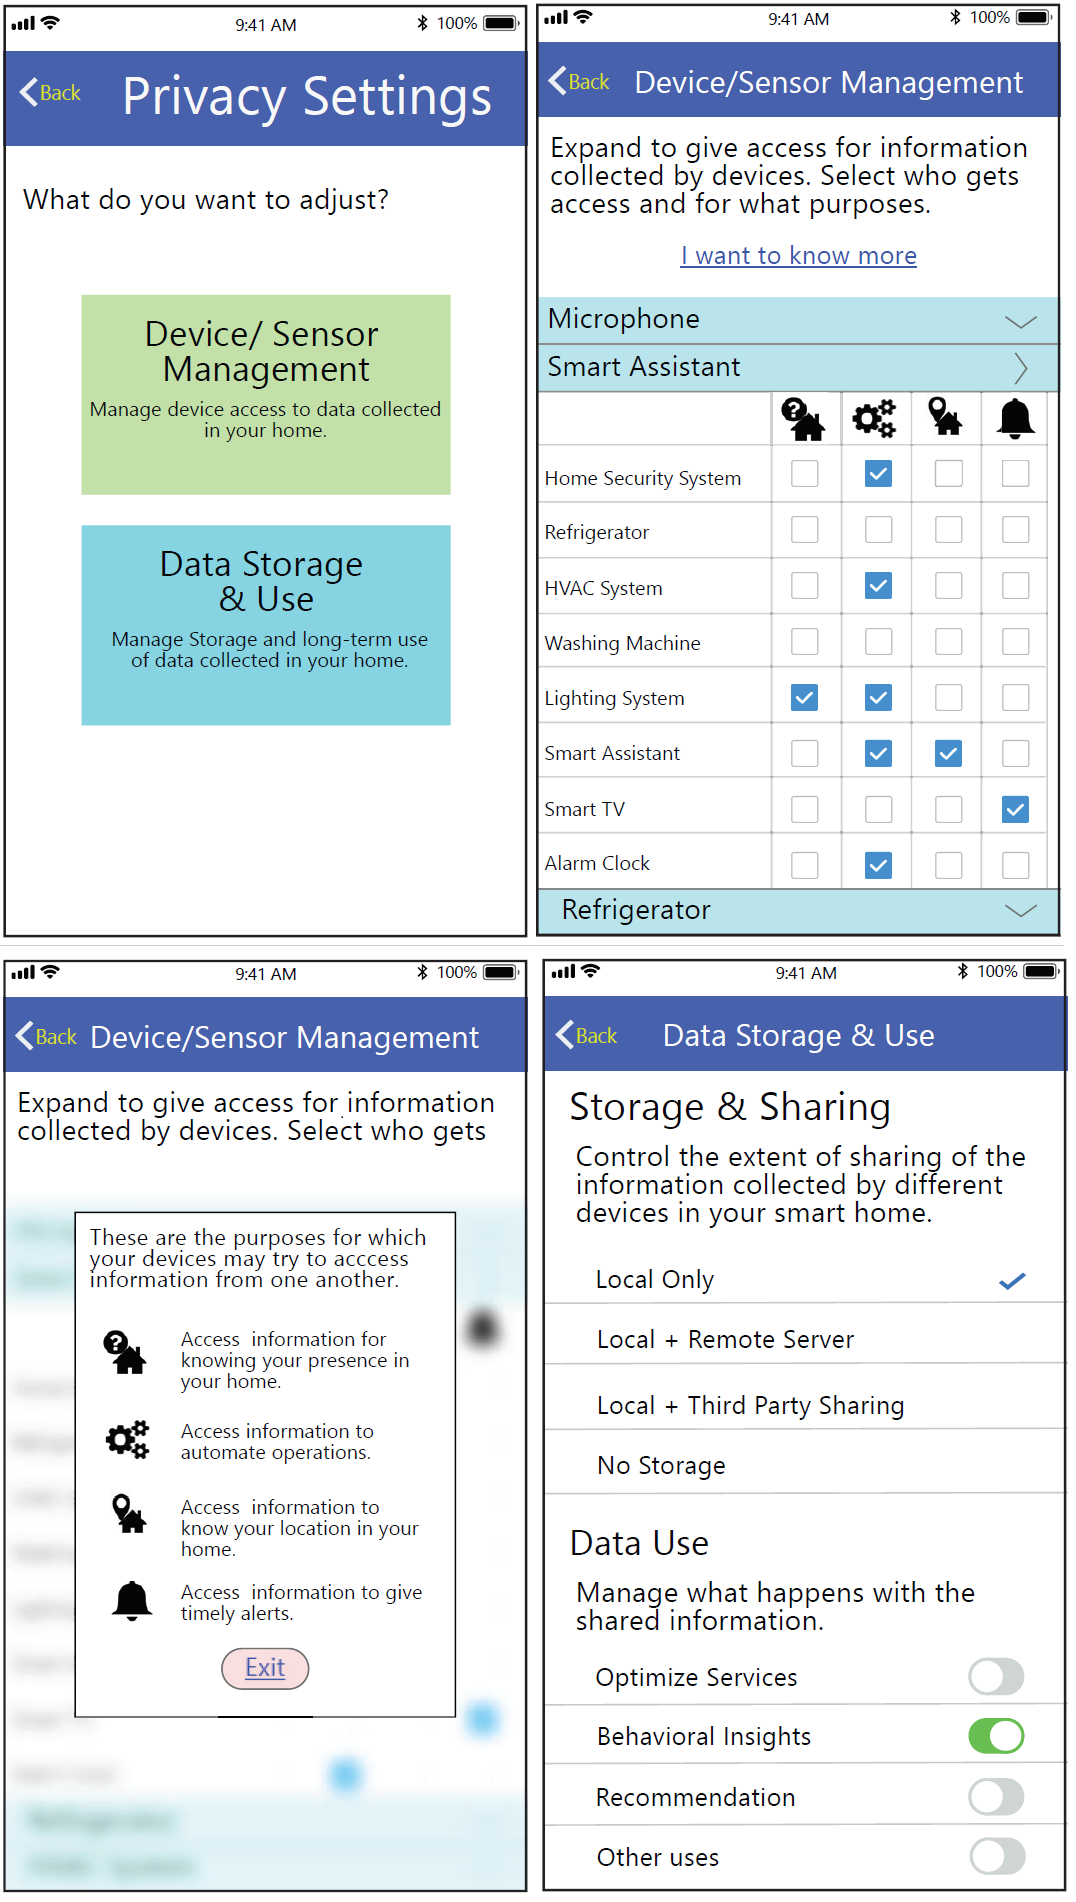
\includegraphics[width=0.7\textwidth]{figures/interface_new.png}
	\caption{Screen 1 (top left) is the landing page of our manual settings interface, screen 2 (top right) is the Device/Sensor Management page, screen 3 (bottom left) shows the explanation when you click on ``I want to learn more'', and screen 4 (bottom right) is the Data Storage \& Use page.}
	\label{fig:interface2}
\end{figure}

\textbf{Device/Sensor Management:} This screen (Figure~\ref{fig:interface2}, screen 2) allows users to control the \emph{Purposes} for which each device (\emph{Who}) is allowed to access data collected by itself, other devices, and the smart home sensors installed around the house (\emph{What}). This screen has a collapsible list of data-collecting devices and sensors (\emph{What}). For each device/sensor, the user can choose what devices can access the collected data (\emph{Who}; in rows), and what it may use that data for (\emph{Purpose}; in columns).

In the example of Figure~\ref{fig:interface2}, the user does not give the `Refrigerator' access to information collected by the `Smart Assistant' for any of the four purposes, while they give the `Smart TV' access to this data for the purpose of giving `timely alerts'. In this example the `Smart Assistant' is allowed to use its own data to `automate operations' and to `know your location in your home'.

Showing \emph{Who}, \emph{What} and \emph{Purpose} at the same time allows users to enable/disable specific combinations of settings---the significant interaction effects between these parameters suggest that this is a necessity. The icons for the \emph{Purpose} requirement allow this settings grid to fit on a smartphone or in-home control panel. We expect that users will quickly learn the meaning of these icons, but they can always click on `I want to know more' to learn their meaning (see Figure~\ref{fig:interface2}, screen 3). 

%If users want to further provide access for specific purpose, then they can click on `More'. Once users tap on `More' they are navigated to Screen-1 of the interface where they can see the different levels of `Purpose' parameter. By showing different levels of `Who' and `What' parameters on Screen-2, we account for the interaction effects between them, the user can now see both the levels at a time thereby making a decision on the grounds of both of these parameters. In Screen-1 we also account for interactions between `Who-What' and `Purpose' because at the bottom of this Screen, users see the flow of information across different device of the former parameters.

%Although, `Purpose' seems to be slightly more important parameter as compared to `Who' and `What', while designing, we envisaged that the interaction effects between `Who' and `What' play a more dominant role and showing different devices involved in the latter parameters would help users gain a quicker grasp over the flow of information in the system.

\textbf{Data Storage \& Use:} This screen (Figure~\ref{fig:interface2}, screen 4) allows users to control how their data is stored and shared (\emph{Storage}), as well as how stored data is used (\emph{Action}). These settings are independent from each other and from the Device/Sensor Management settings. 

For `Storage \& Sharing', users can choose to turn storage off altogether, store data locally, store data both locally and on a remote server, or store data locally and on a remote server \emph{and} allow the app to share the data with third parties. Note that the options for \emph{Storage} are presented as ordered, mutually exclusive settings. Our scenarios did not present them as such (i.e., participants were free to reject local storage but allow remote storage). However, the \emph{Storage} parameter showed a very clear separation of levels%(see Figure~\ref{fig:storage_post} in the Appendix)
, so this presentation is justified. For `Data Use', the users can choose to enable/disable the use of the collected data for various secondary purposes: behavioral insights, recommendations, service optimization, and/or other purposes.

In the subsequent sections we describe the results from our machine learning analysis and further explain how these results impact the designs presented in this section. For this purpose, Section~\ref{sec:design_ml} revisits the interface designs presented here.

\section{Predicting users' behaviors (original work)}\label{sec:predict}
In this section we predict participants' \textit{enable}/\textit{disable} decision using machine learning methods. Similarly, we do not attempt to find the best possible solution; instead we make a conscious trade-off between parsimony and prediction accuracy. Accuracy is important to ensure that users' privacy preferences are accurately captured and/or need only few manual adjustments. Parsimony, on the other hand, prevents overfitting and promotes fairness: we noticed that more complex models tended to increase overall accuracy by predicting a few users' preferences more accurately, with no effect on other users. Parsimony also makes the associated default setting easier to understand for the user.

%Our prediction target is the participants' decision to \textit{enable} or \textit{disable} the data collection described in each scenario. The scenario parameters serve as input attributes. These are nominal variables, making decision tree algorithms such as ID3 and J48 a suitable prediction approach. Unlike ID3, J48 uses gain ratio as the root node selection metric, which is not biased towards input attributes with many values. Moreover, by using J48 decision trees, the amount of pruning for the model can be easily manipulated to investigate the trade-off between the accuracy and parsimony. We therefore use J48 throughout our analysis.

Our prediction target is the participants' decision to \textit{enable} or \textit{disable} the data collection described in each scenario. The scenario parameters serve as input attributes. Using Java and Weka's Java library~\cite{witten2016data} for modeling and evaluation, we implement progressively sophisticated methods for predicting participants' decisions. After discussing naive (enable/disable all) solutions and One Rule Prediction, we first present a cross-validated tree learning solution that results in a single ``smart default'' setting that is the same for everyone. Subsequently, we discuss three different procedures that create a number of ``smart profiles'' by clustering the participants and creating a separate cross-validated tree for each cluster. For each procedure, we try various numbers of clusters and pruning parameters. The solutions with the most parsimonious trees and the highest accuracies of each approach are reported in Table~\ref{tab:comp_approach2}; more detailed results of the parsimony/accuracy trade-off are presented in Figures~\ref{fig:smart_default_optimal}, \ref{fig:attitudesum}, \ref{fig:conglosum} and \ref{fig:fitsum} throughout the paper, and combined in Figure~\ref{fig:summary}.

\newcommand{\specialcell}[2][c]{%
	\begin{tabular}[#1]{@{}c@{}}#2\end{tabular}}

\begin{table}
	\centering
	\caption{Comparison of clustering approaches (highest parsimony and highest accuracy)}
	\label{tab:comp_approach2}
	\begin{tabular}{l|c|c|c|c}
		\hline
		Approach & \specialcell{Inital \\ clusters} & \specialcell{Final \# of \\ profiles} & \specialcell{Complexity \\ (avg. tree size/profile)} & Accuracy \\ \hline
		Naive (enable all) & 1 & 1 & 1 & 46.74\% \\
		Naive (disable all) & 1 & 1 & 1 & 53.26\% \\ \hline
		One Rule (Fig.~\ref{fig:oneR}) & 1 & 1 & 3 & 61.39\% \\ \hline
		\multirow{2}{8em}{Overall (Fig.~\ref{fig:smart_default_optimal})} 
		& 1 & 1 & 8 & 63.32\% \\ 
		& 1 & 1 & 264 & 63.76\% \\ \hline 
		\multirow{6}{8em}{Attitude-based clustering (Fig.~\ref{fig:attitudesum})}
		& 2 & 2 & 2 & 69.44\% \\
		& 2 & 2 & 121.5 & 72.66\% \\ \cdashline{2-5}[.5pt/1pt]
		& 3 & 3 & 2.67 & 72.19\% \\
		& 3 & 3 & 26.67 & 73.47\% \\ \cdashline{2-5}[.5pt/1pt]
		& 5 & 4 & 3 & 72.61\% \\ 
		& 5 & 4 & 26 & 73.56\% \\ \hline
		\multirow{3}{8em}{Agglomerative clustering (Fig.~\ref{fig:conglosum})} & 1133 & 4 & 2 & 79.4\% \\ 
		& 1133 & 5 & 2.4 & 80.35\% \\ 
		& 1133 & 6 & 3.17 & 80.60\% \\ \hline
		\multirow{8}{7.5em}{Fit-based clustering (Fig.~\ref{fig:fitsum})} 
		& 2 & 2 & 2 & 74.43\% \\
		& 2 & 2 & 151.5 & 76.72\% \\ \cdashline{2-5}[.5pt/1pt]
		& 3 & 3 & 7 & 79.80\% \\
		& 3 & 3 & 65.33 & 80.81\% \\ \cdashline{2-5}[.5pt/1pt]
		& 4 & 4 & 9.25 & 81.88\% \\
		& 4 & 4 & 58.25 & 82.41\% \\ \cdashline{2-5}[.5pt/1pt]
		& 5 & 5 & 4.2 & 82.92\% \\
		& 5 & 5 & 51.4 & 83.35\% \\ \hline
	\end{tabular}
\end{table}

\subsection{Naive Prediction Model}
We start with the naive or ``information-less" predictions. Compared to our previous work~\cite{bahiratiui2018}, our current dataset shows that it is even less amenable to a `simple' default setting: it contains 6335 \emph{enable} cases and 7241 \emph{disable} cases, which means that predicting \textit{enable} for every setting gives us a 46.74\% prediction accuracy, while making a \textit{disable} prediction for every setting gives us an accuracy of 53.26\%. In other words, if we disable all information collection by default, only 53.26\% users will on average be satisfied with this default settings. Moreover, such a default setting disallows any `smart home' functionality by default---arguably not a solution the producers of smart appliances can get behind.

\subsection{One Rule Prediction}
Next, we use a ``\textit{One Rule}" (OneR) algorithm to predict users' decision using the simplest prediction model possible. OneR is a very simple but often surprisingly effective learning algorithm~\cite{Holte1993}. It creates a frequency table for each predictor against the target, and then find the best predictor with the smallest total error based on the frequencies.

As shown in Figure~\ref{fig:oneR}, the OneR model predicts users' decision solely based on the \textbf{Storage} parameter with an accuracy of 61.39\%.  Based on this model, if we enable all information-sharing \emph{except} with third parties, we will on average satisfy 61.39\% of users' preferences---a 15.3\% improvement\footnote{61.39 / 53.26 = 1.153} over the naive ``disable all'' default. Note, though, that this default setting is overly permissive, with 3262 false positive predictions (see Table~\ref{tab:oner_confusion_matrix}).

\begin{figure}
	\centering
	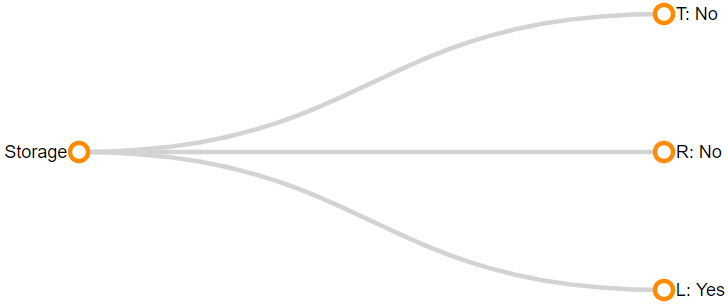
\includegraphics[width=0.6\textwidth]{figures/oneR.png}
	\caption{A ``smart default'' setting based on the ``One Rule" algorithm (4 nodes, accuracy: 61.39\%). Parameter value abbreviations correspond to the ``code'' column in Table~\ref{tab:parameter2}.}
	\label{fig:oneR}
\end{figure}


\begin{table}
	\centering
	\caption{Confusion matrix for the One Rule prediction}
	\label{tab:oner_confusion_matrix}
	\begin{tabular}{c|c|c|c} \hline
		Observed &\multicolumn{2}{c|}{Prediction} & Total\\ \cline{2-3}
		& Enable     & Disable       &  \\ \hline
		Enable   & 5085 (TP) & 1270 (FN)  & 6355   \\ \hline
		Disable    & 3262 (FP)  & 3979 (TN) & 7241  \\ \hline
		Total & 7192     & 6404     & 13596  \\ \hline
	\end{tabular}
\end{table}

\subsection{Overall Prediction}
Moving beyond a single parameter, we create a ``smart default'' setting by predicting the \textit{enable}/\textit{disable} decision with all scenario parameters using the J48 decision tree algorithm.
The resulting tree has an accuracy of 63.76\%. As shown in Figure~\ref{fig:smart_default}, this model predicts users' decision on \textbf{Storage} first. It predicts \textit{disable} for every scenarios with collected data stored on a remote server and shared with third party. For scenarios that store collected data on remote server without sharing, the default settings will depend on the `purpose' of information sharing. There is a further drill down based on `who' and `what'. For scenarios that store collected data locally, the default settings will depend on the `what'. There is a further drill down based on `who', `what', and `action'. With this default setting, users would on average be satisfied with 63.76\% of these settings---a 19.7\% improvement over the naive ``disable all" default. 

\begin{figure}
	\centering
	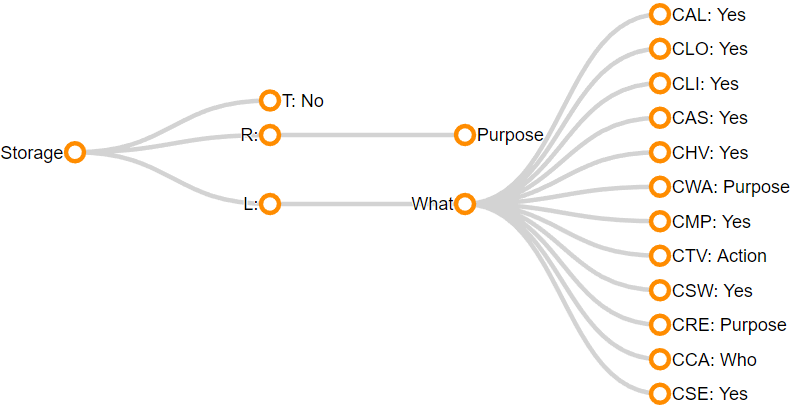
\includegraphics[width=0.7\textwidth]{figures/smartdefault025.png}
	\caption{A ``smart default'' setting with 264 nodes (accuracy: 63.76\%). Parameter value abbreviations correspond to the ``code'' column in Table~\ref{tab:parameter2}.}
	\label{fig:smart_default}
\end{figure}

On the downside, this ``smart default'' setting is quite complex---the ``smart default'' in our previous work~\cite{bahiratiui2018} contained only 49 nodes, whereas the ``smart default'' for our current dataset has 264 nodes. Compared to \textit{One Rule} algorithm, which only has 4 nodes in its decision tree and is thus much easier to explain, the accuracy improvement of Smart Default is only 3.8\%. This highlights the trade-off between parsimony and prediction accuracy that we have to make when developing ``smart default'' settings. On the upside, though, the prediction of the J48 decision tree algorithm is more balanced, with a roughly equal number of false positives and false negatives (see Table~\ref{tab:confusion_matrix2}).


\begin{table}
	\centering
	\caption{Confusion matrix for the overall prediction}
	\label{tab:confusion_matrix2}
	\begin{tabular}{c|c|c|c} \hline
		Observed &\multicolumn{2}{c|}{Prediction} & Total\\ \cline{2-3}
		& Enable     & Disable       &  \\ \hline
		Enable   & 4753 (TP) & 2488 (FN)  & 7241   \\ \hline
		Disable    & 2439 (FP)  & 3916 (TN) & 6355  \\ \hline
		Total & 7192     & 6404     & 13596  \\ \hline
	\end{tabular}
\end{table}

To better understand the parsimony/accuracy trade-off, we vary the degree of model pruning to investigate the effect of increasing the parsimony (i.e., more trimming) on the accuracy of the resulting ``smart default'' setting. The parameter used to alter the amount of post-pruning performed on the J48 decision trees is called Confidence Factor ($CF$) in Weka, and lowering the Confidence Factor will incur more pruning. We tested the J48 classifier with a Confidence Factor ranging from 0.01 to 0.25 (the default setting in Weka) with an increments of 0.01.

Figure~\ref{fig:smart_default_cf} displays the accuracy and the size of the decision tree as a function of the Confidence Factor. The X-axis represents the Confidence Factor; the left Y-axis and the orange line represent the accuracy of the smart default setting; the right Y-axis and the dotted blue line represent the size of the decision tree for that setting. The highest accuracy, 63.75\%, is achieved with the 264-node decision tree produced by $CF = 0.25$. The lowest accuracy, 62.9\%, is achieved with the 44-node decision tree produced by $CF = 0.19$. When $CF \leq 0.16$, the decision tree contains only 8 nodes. The 8-node profile with the highest accuracy is produced by $CF = 0.10$ with an accuracy of 63.32\%.

\begin{figure}
	\centering
	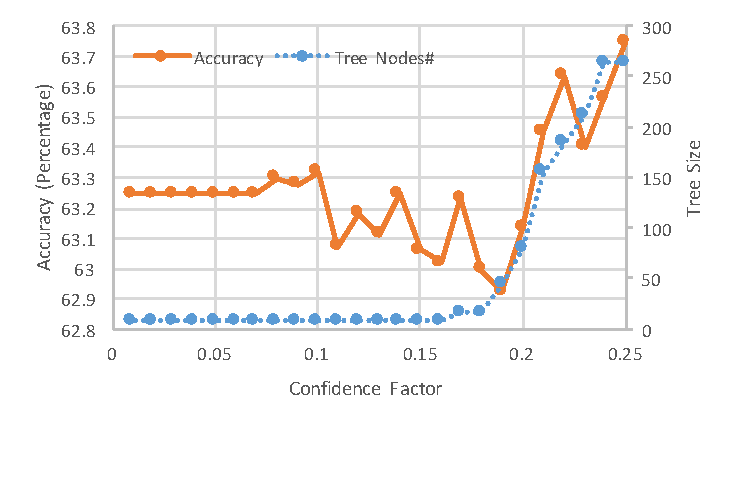
\includegraphics[width=0.65\textwidth]{figures/smart_default_cf.pdf}
	\caption{Accuracy and parsimony (tree size) of the smart default change as a function of Confidence Factor}
	\label{fig:smart_default_cf}
\end{figure}

Figure~\ref{fig:smart_default_optimal} summarizes accuracy as a function of parsimony. The X-axis represents the number number of nodes in the decision tree (more = lower parsimony); the Y-axis represents the accuracy of the decision tree. The figure shows the most accurate J48 solution for any given tree size, and includes the One Rule and Naive predictions for comparison. Reducing the tree from 264 to 8 nodes incurs a negligible 0.67\% reduction in accuracy. This decision tree is shown in Figure~\ref{fig:smart_default_new}, and is still 3.1\% better than the One Rule prediction model and 18.9\% better than the naive ``disable all" default. This more parsimonious ``smart default'' setting  can easily be explained to users as follows: 
\begin{itemize}
	\item All sharing with third parties will be disabled by default. 
	\item Remote storage is allowed for automation and alerts, but not for detecting your presence or location in the house. 
	\item Local storage is allowed for all purposes.
\end{itemize}


\begin{figure}
	\centering
	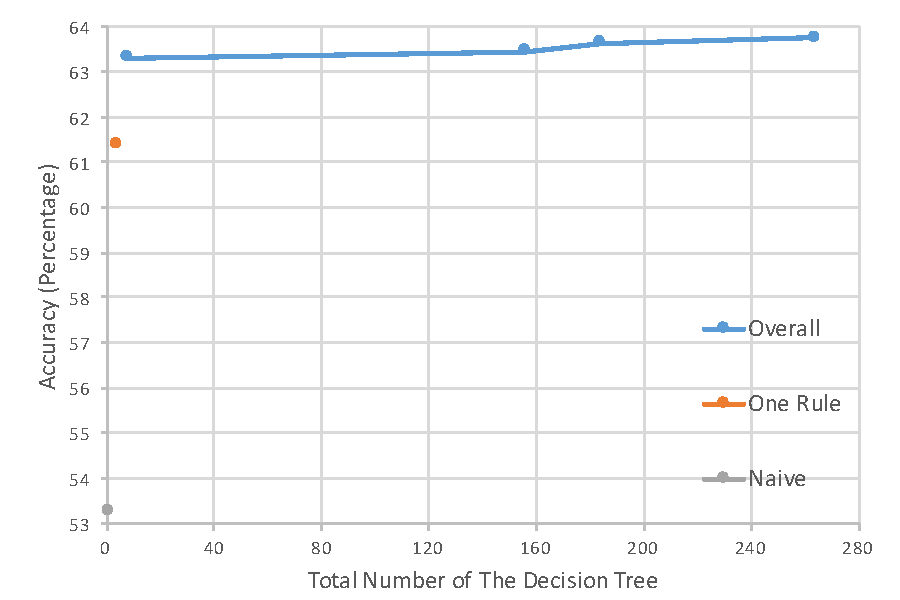
\includegraphics[width=0.6\textwidth]{figures/smart_default_optimal.pdf}
	\caption{Parsimony/accuracy comparison for Naive, One Rule, and Overall Prediction}
	\label{fig:smart_default_optimal}
\end{figure}

\begin{figure}
	\centering
	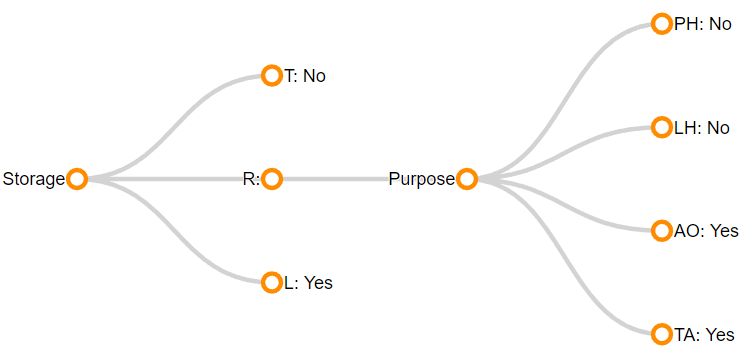
\includegraphics[width=0.6\textwidth]{figures/smartdefault001.png}
	\caption{A ``smart default'' setting with only 8 nodes (accuracy: 63.32\%). Parameter value abbreviations correspond to the ``code'' column in Table~\ref{tab:parameter2}.}
	\label{fig:smart_default_new}
\end{figure}


While the ``smart default'' setting makes a considerable improvement over a naive default, there is still a lot of room for improvement---even our best prediction model only correctly models on average 63.76\% of the user's desired settings. This should come at no surprise, as one of the most consistent findings in the field of privacy is that people differ substantially in their privacy preferences~\cite{knijnenburg2013dimensionality}. As a result, our ``one-size fits all'' default setting---smart as it may be---is not very accurate. Recent work in the field of privacy suggest to \emph{tailor} the privacy settings to the user to accommodate for these interpersonal differences~\cite{knijnenburg2017}. Our previous work therefore moved beyond ``smart default'' settings by clustering participants with similar privacy preferences and creating a set of ``smart profiles'' covering each of the clusters~\cite{bahiratiui2018}. The idea is that the accuracy of the tree for each cluster will likely exceed the accuracy of our overall prediction model. 

In the remainder of this section we apply existing and new clustering methods with the aim of creating separate ``smart profiles" for each cluster. As our goal is to develop simple, understandable profiles, we keep the parsimony/accuracy trade-off in mind during this process.


\subsection{Attitude-Based Clustering}
%As shown in Figure~\ref{fig:mediation_test}, 
Our statistical results indicate that the effects of scenario parameters on users' decisions are mediated by their attitudes (Risk, Comfort, Appropriateness, Expectedness and Usefulness). Therefore, our first attempt to develop ``smart profiles'' is to cluster participants with similar attitudes towards the 12 scenarios they evaluated. We averaged the values per attitude across each participant's 12 answers, and ran a \textit{k-means} clustering algorithm to divide them into 2, 3, 4, 5, and 6 clusters. We then added the participants' cluster assignments back to our original dataset, and ran the J48 decision tree algorithm on the dataset with this additional \emph{Cluster} attribute for each number of clusters, varying the Confidence Factor from 0.01 to 0.25 with increments of 0.01. The results are summarized in Figure~\ref{fig:attitudesum}, which displays the most accurate solution for any given tree size and number of clusters.

%Actual profile numbers, average tree sizes per profile, and accuracies for resulting solutions are reported in Table~\ref{tab:attitude_results}.

All of the resulting decision trees have \emph{Cluster} as the root node. This justifies our approach, because it indicates that the \emph{Cluster} parameter is a very effective for predicting users' decisions. It also allows us to split the decision trees at the root node, and a create different ``smart profile'' for each subtree/cluster. Note that for some solutions two clusters end up with the same decision tree, which effectively reduces the number of profiles by 1.

\begin{figure}
	\centering
	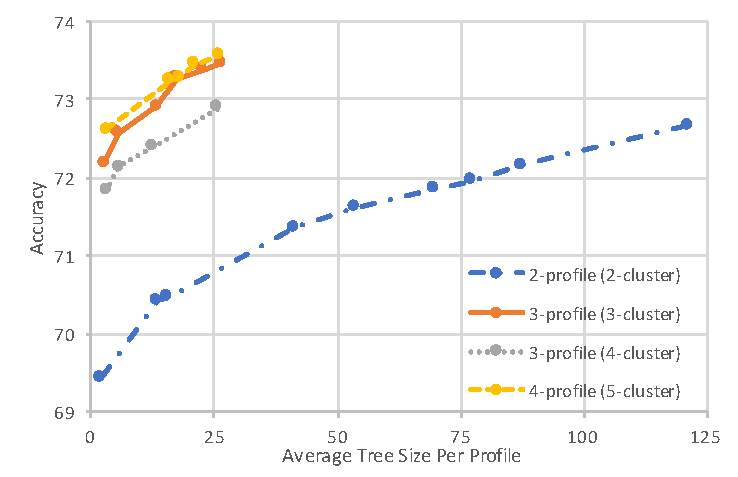
\includegraphics[width=0.95\textwidth]{figures/attitudeSum2.pdf}
	\caption{Parsimony/accuracy comparison for attitude-based clustering}
	\label{fig:attitudesum}
\end{figure}

%\begin{table}
%	\centering
%	\caption{Attitude Clustering Results}
%	\label{tab:attitude_results}
%	\begin{tabular}{c||c|c|c||c|c|c||c|c|c||c|c|c} \hline
%	&  \multicolumn{3}{c||}{2-cluster} & \multicolumn{3}{c||}{3-cluster} & \multicolumn{3}{c||}{4-cluster}  & \multicolumn{3}{c}{5-cluster} \\ \hline
%	Confi- &  & Avg & Accu- &  & Avg & Accu- &  & Avg & Accu- &  & Avg & Accu- \\
%	dence  &  & tree & racy &  & tree & racy &  & tree & racy &  & Tree & racy \\
%	  & * & size &  & * & size &  & * & size &  & * & size &  \\ 
%	Factor &  & /prof. &  &  & /prof. & &  & /prof. & &  & /prof. \\ \hline
%0.01 & 2 & 3 & 69.44\% & 3 & 3.67 & 72.19\% & 3 & 4 & 71.82\% & 4 & 4 & 72.61\% \\
%0.02 & 2 & 3 & 69.44\% & 3 & 6.33 & 72.57\% & 3 & 4 & 71.82\% & 4 & 4 & 72.61\% \\
%0.03 & 2 & 3 & 69.44\% & 3 & 6.33 & 72.57\% & 3 & 4 & 71.82\% & 4 & 4 & 72.61\% \\
%0.04 & 2 & 3 & 69.44\% & 3 & 6.33 & 72.57\% & 3 & 6.67 & 72.14\% & 4 & 4 & 72.61\% \\
%0.05 & 2 & 3 & 69.44\% & 3 & 6.33 & 72.57\% & 3 & 6.67 & 72.14\% & 4 & 4 & 72.61\% \\
%0.06 & 2 & 3 & 69.44\% & 3 & 6.33 & 72.57\% & 3 & 6.67 & 72.14\% & 4 & 4 & 72.61\% \\
%0.07 & 2 & 3 & 69.44\% & 3 & 6.33 & 72.57\% & 3 & 6.67 & 72.14\% & 4 & 4 & 72.61\% \\
%0.08 & 2 & 3 & 69.44\% & 3 & 6.33 & 72.57\% & 3 & 6.67 & 72.14\% & 4 & 4 & 72.61\% \\
%0.09 & 2 & 3 & 69.44\% & 3 & 6.33 & 72.57\% & 3 & 6.67 & 72.14\% & 4 & 4 & 72.61\% \\
%0.1 & 2 & 14.5 & 70.43\% & 3 & 6.33 & 72.57\% & 3 & 6.67 & 72.14\% & 4 & 4 & 72.61\% \\
%0.11 & 2 & 14.5 & 70.43\% & 3 & 6.33 & 72.57\% & 3 & 6.67 & 72.14\% & 4 & 4 & 72.61\% \\
%0.12 & 2 & 14.5 & 70.43\% & 3 & 6.33 & 72.57\% & 3 & 6.67 & 72.14\% & 4 & 4 & 72.61\% \\
%0.13 & 2 & 14.5 & 70.43\% & 3 & 6.33 & 72.57\% & 3 & 6.67 & 72.14\% & 4 & 4 & 72.61\% \\
%0.14 & 2 & 14.5 & 70.43\% & 3 & 6.33 & 72.57\% & 3 & 6.67 & 72.14\% & 4 & 4 & 72.61\% \\
%0.15 & 2 & 16.5 & 70.47\% & 3 & 6.33 & 72.57\% & 3 & 6.67 & 72.14\% & 4 & 4 & 72.61\% \\
%0.16 & 2 & 16.5 & 70.47\% & 3 & 14.33 & 72.91\% & 3 & 6.67 & 72.14\% & 4 & 4 & 72.61\% \\
%0.17 & 2 & 16.5 & 70.47\% & 3 & 18.33 & 73.26\% & 3 & 6.67 & 72.14\% & 4 & 4 & 72.61\% \\
%0.18 & 2 & 42.5 & 71.37\% & 3 & 18.33 & 73.26\% & 3 & 6.67 & 72.14\% & 4 & 4 & 72.61\% \\
%0.19 & 2 & 54.5 & 71.62\% & 3 & 18.33 & 73.26\% & 3 & 6.67 & 72.14\% & 4 & 4 & 72.61\% \\
%0.2 & 2 & 54.5 & 71.62\% & 3 & 18.33 & 73.26\% & 3 & 6.67 & 72.14\% & 4 & 17 & 73.24\% \\
%0.21 & 2 & 70.5 & 71.85\% & 3 & 23.67 & 73.37\% & 3 & 13.33 & 72.39\% & 4 & 17 & 73.24\% \\
%0.22 & 2 & 78.5 & 71.96\% & 3 & 27.67 & 73.47\% & 3 & 13.33 & 72.39\% & 4 & 19 & 73.29\% \\
%0.23 & 2 & 88.5 & 72.16\% & 3 & 27.67 & 73.47\% & 3 & 13.33 & 72.39\% & 4 & 22 & 73.46\% \\
%0.24 & 2 & 88.5 & 72.16\% & 3 & 27.67 & 73.47\% & 3 & 13.33 & 72.39\% & 4 & 22 & 73.46\% \\
%0.25 & 2 & 122.5 & 72.66\% & 3 & 27.67 & 73.47\% & 3 & 26.67 & 72.90\% & 4 & 27 & 73.56\% \\ \hline
%	\end{tabular}
%\bigskip
%\footnotesize
%
%\textbf{$*$}: Actual Profile Number.
%\end{table}

%As shown in Table~\ref{tab:attitude_results}, as the Confidence Factor increases from 0.01 to 0.25, the actual resulting profile number of 2-cluster solution keeps at 2, 
For the 2-cluster solutions (the blue line in Figure~\ref{fig:attitudesum}), the highest accuracy is 72.66\%, which is a 14.0\% improvement over the best single ``smart default'' setting. However, this tree has an average of 121.5 nodes per profile. In comparison, the most parsimonious solution has only 1 node (``disable all'') for one of the clusters, and 3 nodes (``disable sharing with third parties'') for the other cluster (see Figure~\ref{fig:att_2_profile}). This solution still has an accuracy of 69.44\%, which is still an 8.9\% increase over the best single ``smart default'' setting.

\begin{figure}
	\centering
	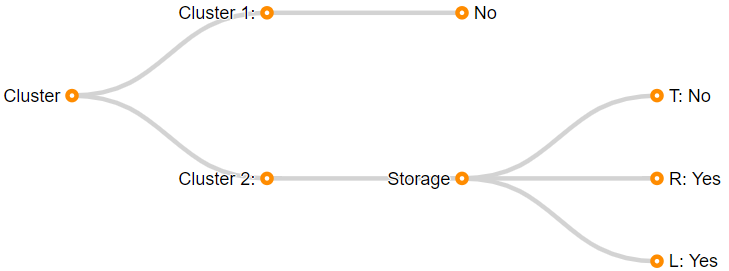
\includegraphics[width=0.8\textwidth]{figures/fit_2_profile001.png}
	\caption{The most parsimonious 2-profile attitude-based solution (2 nodes/profile, accuracy: 69.44\%). Parameter value abbreviations correspond to the ``code'' column in Table~\ref{tab:parameter2}.}
	\label{fig:att_2_profile}
\end{figure}

For the 3-cluster solutions (the orange line in Figure~\ref{fig:attitudesum}), the highest accuracy of 73.47\% is achieved by a set of trees with 26.67 nodes on average (a minimal improvement of 1.1\% over the best 2-cluster solution, but with simpler trees), while the most parsimonious solution has a ``disable all'' and an ``enable all'' tree, plus a tree that is the same as the most parsimonious smart default setting (see Figure~\ref{fig:smart_default_new}). This solution has an accuracy of 72.19\%, which is a 4.0\% increase over the most parsimonious 2-cluster solution.

The 4-cluster solutions (the grey line in Figure~\ref{fig:attitudesum}) all result in ``over-clustering'': all solutions based on the 4-cluster \emph{Cluster} parameter result in two profiles with the same subtree, effectively resulting in a 3-profile solution. The accuracy of these solutions is actually lower than the accuracy of similar 3-cluster solutions, so we will not discuss them here.

The 5-cluster solutions (the yellow line in Figure~\ref{fig:attitudesum}) are also ``over-clustered'', resulting in 4 profiles. The highest accuracy of 73.56\% is achieved by a set of trees with 26 nodes---this is about the same accuracy and parsimony as the most accurate 3-cluster solution. The same holds for the most parsimonious 5-cluster solution, which has a similar accuracy and parsimony as the most parsimonious 3-cluster solution.

The accuracy of the 6-cluster solutions (which result in either 4- or 5-profile solutions) is lower than the accuracy of similar 5-cluster solutions. Therefore, we will not further discuss these results.

Reflecting upon the attitude-based clustering results, we observe in Figure~\ref{fig:attitudesum} that there is indeed a trade-off between accuracy and parsimony: the most parsimonious results are less accurate, but the most accurate results are more complex. Moreover, the 2-profile solutions are about 5\% less accurate than the 3-profile solutions at any level of complexity. The 4-profile solutions do not improve the solution much further, though.

The 3-profile solution with an average of 18.33 nodes per profile and 73.26\% accuracy provides a nice compromise between accuracy and parsimony. Part of this decision tree is shown in Figure~\ref{fig:attitude_3profile}: it contains one ``disable all'' profile, one ``enable all'' profile, and a more complex profile with 55 nodes that disallows sharing with third parties and allows remote and local storage depending on the purpose (not further shown).

\begin{figure}
	\centering
	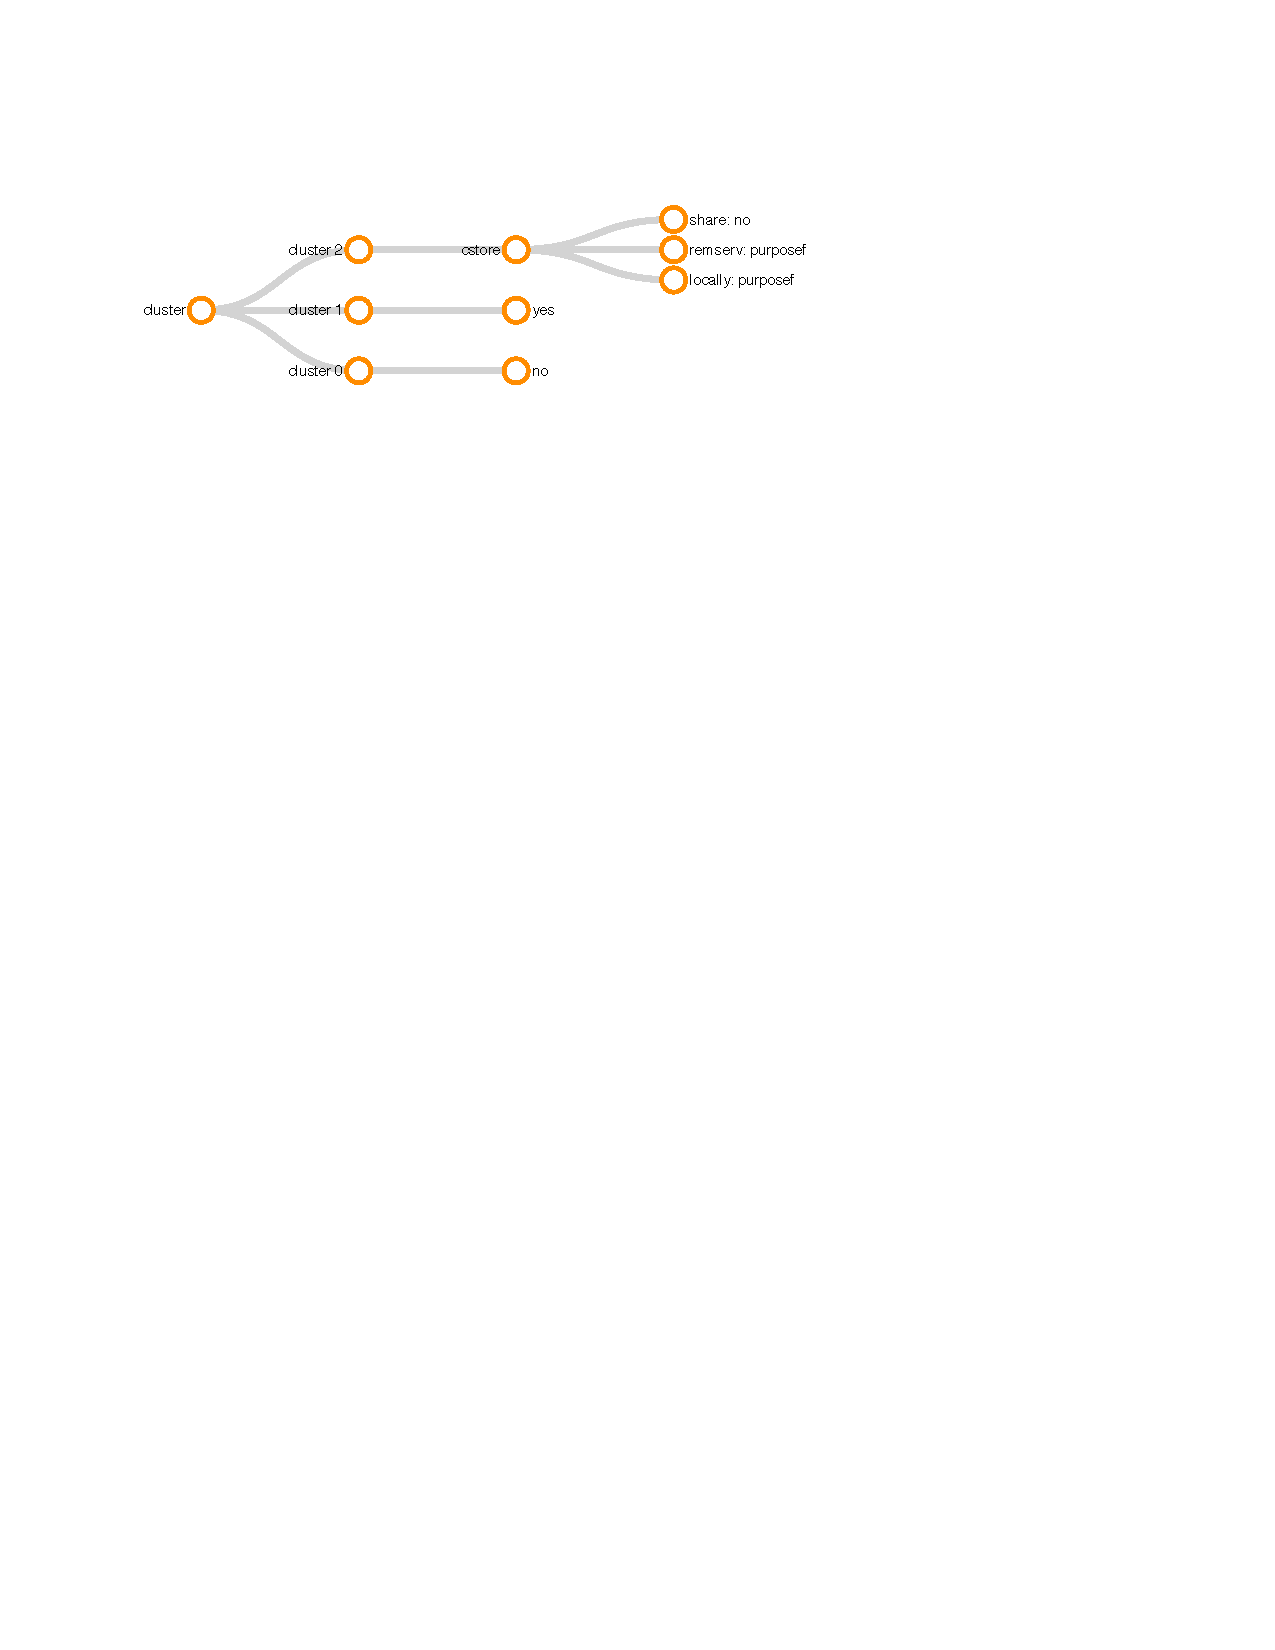
\includegraphics[width=0.7\textwidth]{figures/attitude_3_profile.pdf}
	\caption{A 3-profile solution example of attitude-based clustering (18.33 nodes/profile, accuracy: 73.26\%). Parameter value abbreviations correspond to the ``code'' column in Table~\ref{tab:parameter2}.}
	\label{fig:attitude_3profile}
\end{figure}

\subsection{Agglomerative Clustering}
The attitude-based clustering approach requires knowledge of users' attitudes towards the household IoT information-sharing scenarios, which may not always be available. We developed an alternative method for finding ``smart profiles'' that follows a hierarchical bottom-up (or agglomerative) approach, using users' decisions only. This method first fits a separate decision tree for each participant, and then iteratively merges these trees based on similarity. In our previous work~\cite{bahiratiui2018} only 10 out of the 200 users in the dataset had unique trees fitted to them (all others had an ``enable all'' or ``disable all'' tree), making the merging of trees a rather trivial affair. Our current dataset has many more participants, and is more complex, making the agglomerative clustering approach more challenging but also more meaningful. 

In the first step, 283 participants' decision trees predict ``enable all'', 414 participants' decision trees predict ``disable all'', while the remaining 436 participants have a multi-node decision tree.

In the second step, a new decision tree is generated for each possible pair of participants in the ``multi-node group''. The accuracy of the new tree is compared against the weighted average of the accuracies of the original trees. The pair with smallest reduction in accuracy is merged, leaving 435 clusters for the next round of merging. If two or more candidate pairs have the same smallest reduction in accuracy, priority is given to the pair with the most parsimonious resulting tree (i.e., with smallest number of nodes). If there are still multiple pairs that tie on this criterion, the first pair is picked. The second step is repeated until it reaches the predefined number of clusters, and the entire procedure is repeated with 20 random starts to avoid local optima.

%\begin{table}
%	\centering
%	\caption{Agglomerative Clustering Results for \textit{Multi-node Group}}
%	\label{tab:conglo_results}
%	\begin{tabular}{c||c|c||c|c||c|c} \hline
%	Confi- &  \multicolumn{2}{c||}{4-cluster} & \multicolumn{2}{c||}{5-cluster} & \multicolumn{2}{c}{6-cluster}  \\ \cline{2-7}
%	dence & Average & Accuracy & Average & Accuracy & Average & Accuracy\\
%	Factor & Nodes/Profile & & Nodes/Profile &  & Nodes/Profile &\\ \hline
%	0.01 & 2.5 & 79.40\% & 3 & 80.35\% & 3.83 & 80.68\% \\
%	0.02 & 2.5 & 79.29\% & 3 & 80.26\% & 3.33 & 80.60\% \\
%	0.03 & 2.5 & 79.23\% & 3 & 80.29\% & 3.83 & 80.66\% \\
%	0.04 & 2.5 & 79.23\% & 3 & 80.23\% & 3.83 & 80.60\% \\
%	0.05 & 2.5 & 79.31\% & 3 & 80.23\% & 3.83 & 80.48\% \\
%	0.06 & 2.5 & 79.29\% & 3 & 80.11\% & 3.83 & 80.59\% \\
%	0.07 & 2.5 & 79.39\% & 3 & 80.13\% & 3.83 & 80.56\% \\
%	0.08 & 2.5 & 79.29\% & 3 & 80.13\% & 4.50 & 80.56\% \\
%	0.09 & 2.5 & 79.31\% & 3 & 80.05\% & 3.83 & 80.43\% \\
%	0.10 & 2.5 & 79.27\% & 3 & 79.86\% & 3.83 & 80.32\% \\
%	0.11 & 2.5 & 79.21\% & 3.6 & 79.81\% & 4.50 & 80.59\% \\
%	0.12 & 2.5 & 79.21\% & 3 & 79.94\% & 4.50 & 80.59\% \\
%	0.13 & 2.5 & 79.14\% & 3 & 79.71\% & 4.33 & 79.96\% \\
%	0.14 & 2.5 & 79.18\% & 3.6 & 79.80\% & 4.50 & 80.26\% \\
%	0.15 & 2.5 & 78.99\% & 3 & 79.85\% & 5.67 & 79.96\% \\
%	0.16 & 2.5 & 79.08\% & 3.6 & 79.61\% & 6.83 & 80.59\% \\
%	0.17 & 2.5 & 78.99\% & 3.6 & 79.70\% & 9.83 & 79.81\% \\
%	0.18 & 2.5 & 78.94\% & 3.6 & 79.73\% & 5.83 & 80.15\% \\
%	0.19 & 7.5 & 78.62\% & 7.6 & 79.31\% & 9.83 & 79.71\% \\
%	0.2 & 6.5 & 78.56\% & 13 & 79.19\% & 11.67 & 79.23\% \\
%	0.21 & 4.5 & 78.56\% & 11 & 79.01\% & 9.67 & 79.68\% \\
%	0.22 & 6.5 & 78.49\% & 8.4 & 79.06\% & 8.33 & 79.68\% \\
%	0.23 & 6.5 & 78.81\% & 11.8 & 79.17\% & 15.67 & 79.66\% \\
%	0.24 & 6.5 & 78.87\% & 13.2 & 78.97\% & 13.00 & 79.51\% \\
%	0.25 & 11.5 & 78.41\% & 17.2 & 78.80\% & 11.67 & 79.41\% \\ \hline
%	\end{tabular}
%\end{table}


To fit the trees, we use the J48 classifier with a Confidence Factor ranging from 0.01 to 0.25 with increments of 0.01. Surprisingly, smaller tree sizes result in a \emph{higher} accuracy for agglomerative clustering (see Figure~\ref{fig:conglosum}). This suggests that without extensive trimming, our agglomerative approach arguably overfits the data, resulting in a lower level of cross-validated accuracy.

\begin{figure}
	\centering
	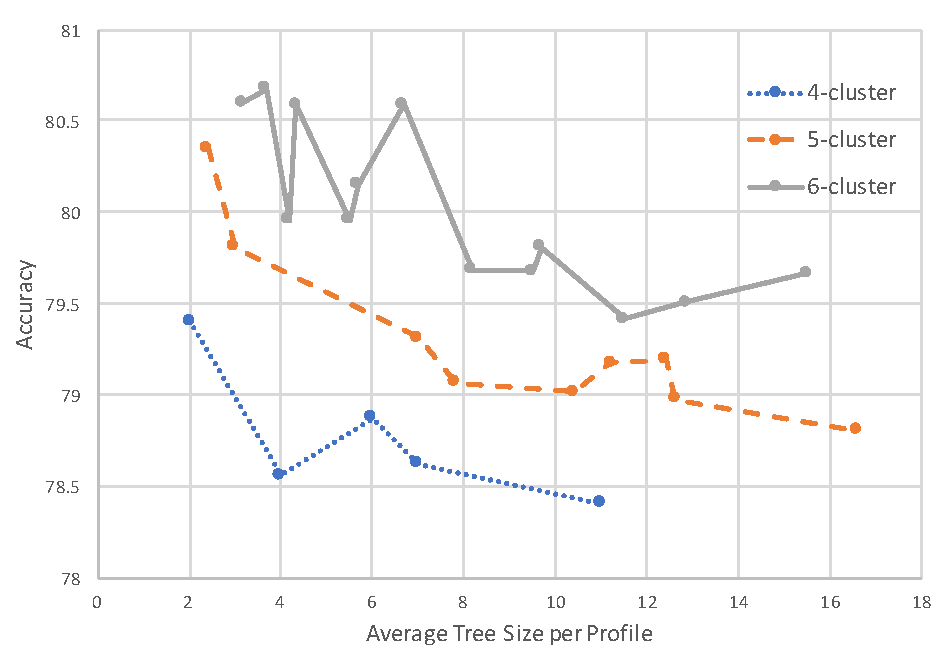
\includegraphics[width=0.7\textwidth]{figures/congloSum2.pdf}
	\caption{Parsimony/accuracy comparison for agglomerative clustering}
	\label{fig:conglosum}
\end{figure}

The best 4-cluster solution has an average of 2 nodes per profile and an accuracy of 79.40\%---a 24.53\% improvement over the ``smart default'', and a 7.9\% increase over the most accurate 5-cluster/4-profile attitude-based clustering solution. The decision trees are shown in Figure~\ref{fig:conglo_4_profile001}: aside from the ``enable all'' and ``disable all'' profiles, there  is a ``disable sharing with third parties'' profile and a ``local storage only'' profile.

\begin{figure}
	\centering
	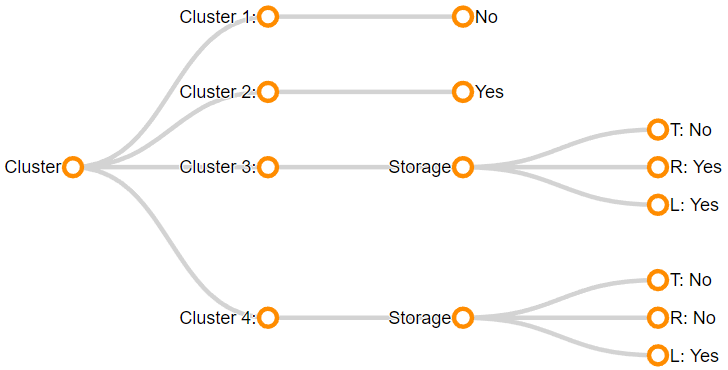
\includegraphics[width=0.6\textwidth]{figures/conglo_4_profile001.png}
	\caption{The best 4-profile agglomerative clustering solution (2 nodes/profile, accuracy: 79.40\%). Parameter value abbreviations correspond to the ``code'' column in Table~\ref{tab:parameter2}.}
	\label{fig:conglo_4_profile001}
\end{figure}

The best 5-cluster solution has an average of 2.4 nodes per profile and an accuracy of 80.35\%---a 26.02\% improvement over the ``smart default'', but only a 1.2\% improvement over the 4-cluster agglomerative solution. The decision trees are shown in Figure~\ref{fig:conglo_5_profile001}: it has the same profiles as the 4-cluster solution, plus an ``allow automation and alerts, but don't track my presence or location in the house'' profile.

\begin{figure}
	\centering
	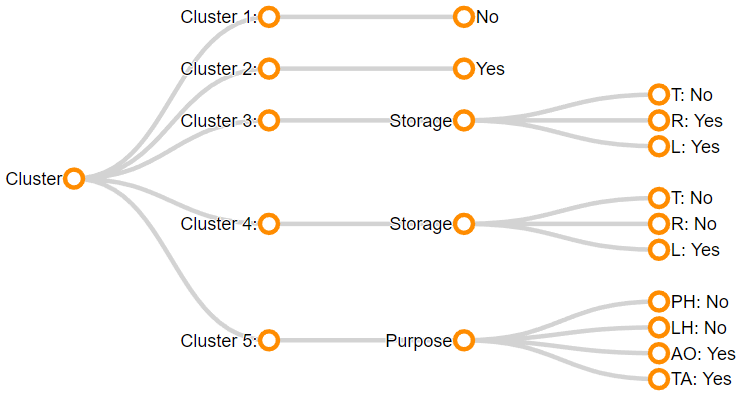
\includegraphics[width=0.6\textwidth]{figures/conglo_5_profile001.png}
	\caption{The best 5-profile agglomerative clustering solution (2.4 nodes/profile, Accuracy: 80.35\%). Parameter value abbreviations correspond to the ``code'' column in Table~\ref{tab:parameter2}.}
	\label{fig:conglo_5_profile001}
\end{figure}

Finally, the best 6-cluster solution\footnote{There is another solution with slightly fewer nodes per profile (2.67) and a slightly lower accuracy (80.60\%).} has an average of 3.17 nodes per profile and an accuracy of 80.68\%---a 26.54\% improvement over the ``smart default'', but no substantial improvement over the 5-cluster agglomerative solution. The decision trees are shown in Figure~\ref{fig:conglo_6_profile001}: it has the same profiles as the 5-cluster solution, plus a profile that allows local storage for anything, plus remote storage for any reason except for user profiling (i.e., to recommend other services or to give the user insight in their behavior).

\begin{figure}
	\centering
	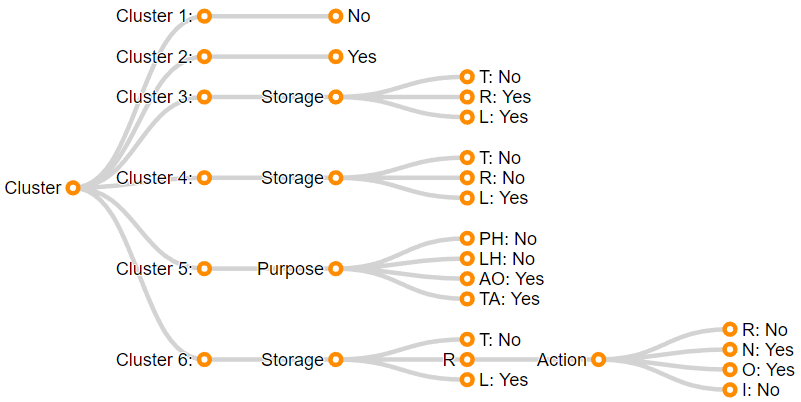
\includegraphics[width=0.6\textwidth]{figures/conglo_6_profile001.png}
	\caption{The best 6-profile agglomerative clustering solution (3.17 nodes/profile, Accuracy: 80.68\% ). Parameter value abbreviations correspond to the ``code'' column in Table~\ref{tab:parameter2}.}
	\label{fig:conglo_6_profile001}
\end{figure}

\subsection{Fit-Based Clustering}
We now present a ``fit-based'' clustering approach that, like the agglomerative approach, clusters participants without using any additional information. Instead, it uses the fit of the tree models to bootstrap the process of sorting participants into different clusters. The steps of our algorithm are as follows:
\begin{itemize}
	\item \textbf{Random starts:} We randomly divide participants into $k$ separate groups, and learn a tree for each group. This is repeated until a non-trivial starting solution (i.e., with distinctly different trees per group) is found. 
	
	\item \textbf{Iterative improvements:} Once each of the $k$ groups has a unique decision tree, we test for each participant which of the $k$ trees best represents their 12 decisions. If this is the tree of a different group, we switch the participant to this group. Once all participants are evaluated and put in the group of their best-fitting tree, the tree in each group is re-learned with the data of the new group members. This then prompts another round of evaluations, and this process continues until no further switches are performed.
	
	\item \textbf{Repeat}: Since this process is influenced by random chance, it is repeated 1,000 times in its entirety to find the optimal solution. Cross-validation is performed in the final step to prevent over-fitting.
\end{itemize}

We perform this approach to obtain 2-, 3-, 4-, and 5-cluster solutions. To fit the trees, we use the J48 classifier with a Confidence Factor ranging from 0.01 to 0.25 with increments of 0.01. The best results are summarized in Figure~\ref{fig:fitsum}.

\begin{figure}
	\centering
	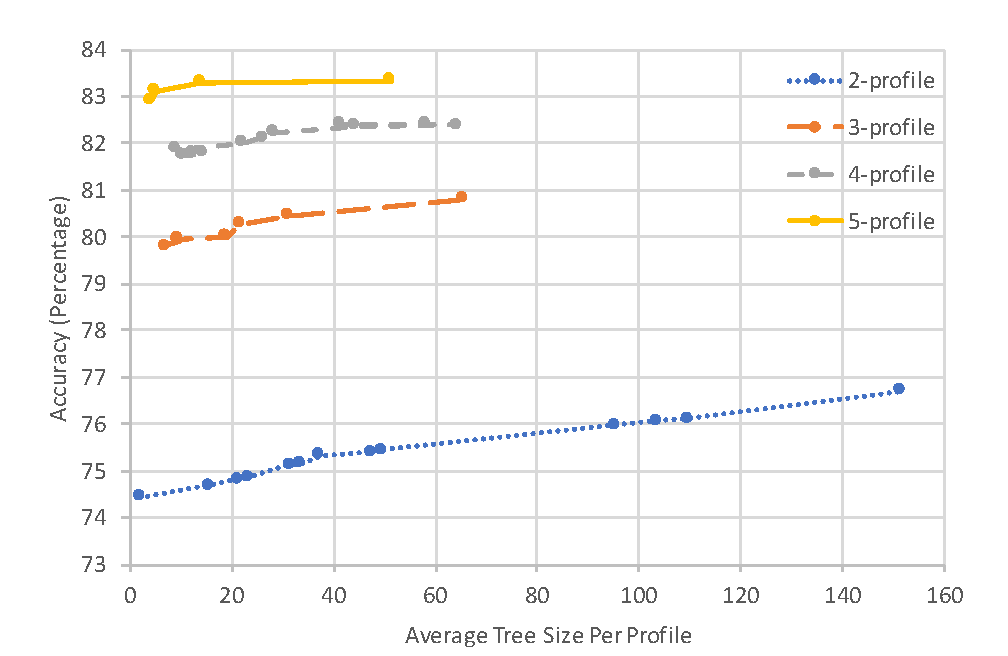
\includegraphics[width=0.7\textwidth]{figures/fitSum.pdf}
	\caption{Parsimony/accuracy comparison for fit-based clustering}
	\label{fig:fitsum}
\end{figure}

For the 2-cluster solutions (the blue line in Figure~\ref{fig:fitsum}), the highest accuracy is 76.72\%---a 20.33\% improvement over the ``smart default'' setting and a 5.6\% improvement over the most accurate 2-cluster attitude-based solution. However, this tree has an average of 151.5 nodes per profile. The most parsimonious solution is exactly the same as the most parsimonious 2-cluster attitude-based solution (see Figure~\ref{fig:att_2_profile}), but with a higher accuracy (74.43\%).

For the 3-cluster solutions (the orange line in Figure~\ref{fig:fitsum}), the highest accuracy of 80.81\% is achieved by a set of trees with 65.33 nodes on average. This is a 26.74\% improvement over the ``smart default'', a 10.0\% improvement over the most accurate 3-cluster attitude-based solution (but at a cost of lower parsimony), and a 5.2\% improvement over the best 2-cluster fit-based solution. The most parsimonious solution, on the other hand, has 7 nodes on average, with an accuracy of 79.80\%, thereby still outperforming all other 3-profile solutions. The decision trees for this solution are shown in Figure~\ref{fig:fit_3_profile001}.

\begin{figure}
	\centering
	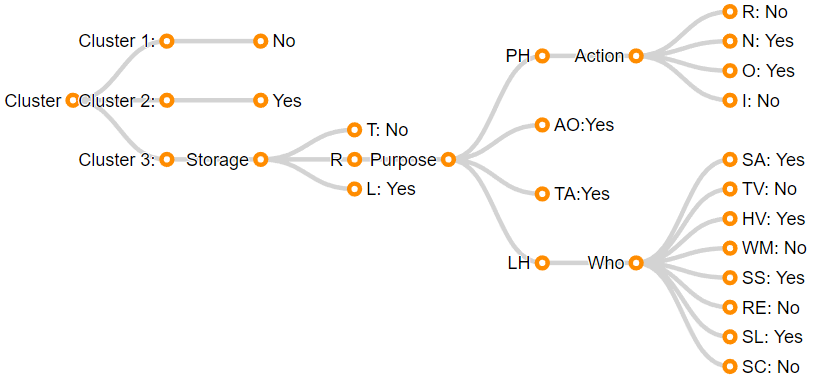
\includegraphics[width=0.6\textwidth]{figures/fit_3_profile001.png}
	\caption{The most parsimonious 3-profile fit-based solution (7 nodes/profile, accuracy: 79.80\%). Parameter value abbreviations correspond to the ``code'' column in Table~\ref{tab:parameter2}.}
	\label{fig:fit_3_profile001}
\end{figure}

For the 4-cluster solutions (the grey line in Figure~\ref{fig:fitsum}), the highest accuracy of 82.41\% is achieved by a set of trees with 58.25 nodes on average. This is a 29.25\% improvement over the ``smart default'', a 3.8\% improvement over the 4-cluster agglomerative solution (but at a cost of lower parsimony), and a 2.0\% improvement over the best 3-cluster fit-based solution. The most parsimonious solution, on the other hand, has 9.25 nodes on average, with an accuracy of 81.88\%. It still outperforms all other 4-profile solutions, but the agglomerative solution is more parsimonious. The decision trees for this solution are shown in Figure~\ref{fig:fit_4_profile010}.

\begin{figure}
	\centering
	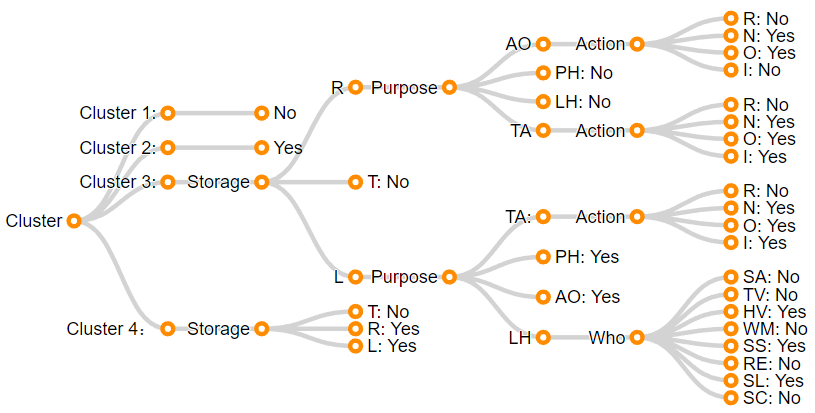
\includegraphics[width=0.6\textwidth]{figures/fit_4_profile010.png}
	\caption{The most parsimonious 4-profile fit-based solution (9.25 nodes/profile, accuracy: 81.88\% ). Parameter value abbreviations correspond to the ``code'' column in Table~\ref{tab:parameter2}.}
	\label{fig:fit_4_profile010}
	\vspace{20px}
\end{figure}

For the 5-cluster solutions (the yellow line in Figure~\ref{fig:fitsum}), the highest accuracy of 83.35\% is achieved by a set of trees with 51.4 nodes on average. This is a 30.05\% improvement over the ``smart default'', a 3.8\% improvement over the 5-cluster agglomerative solution (but at a cost of lower parsimony), and a 1.1\% improvement over the best 4-cluster fit-based solution. The most parsimonious solution, on the other hand, has 4.2 nodes on average, with an accuracy of 82.92\%. It still outperforms the 5-profile agglomerative solution, but it is slightly less parsimonious. The decision trees for this solution are shown in Figure~\ref{fig:fit_5_profile001}.

\begin{figure}
	\centering
	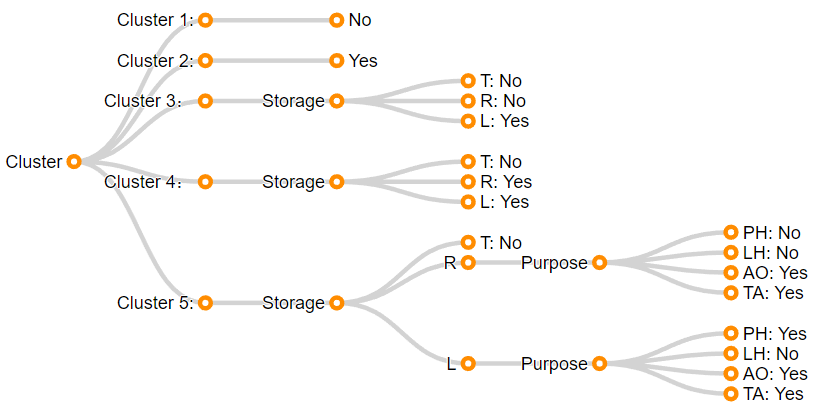
\includegraphics[width=0.6\textwidth]{figures/fit_5_profile001.png}
	\caption{The most parsimonious 5-profile fit-based solution (4.2 nodes/profile, accuracy: 82.92\% ). Parameter value abbreviations correspond to the ``code'' column in Table~\ref{tab:parameter2}.}
	\label{fig:fit_5_profile001}
\end{figure}

%\begin{table}
%	\centering
%	\caption{Fit-Based Clustering Results}
%	\label{tab:fit_results}
%	\begin{tabular}{c||c|c||c|c||c|c||c|c} \hline
%		 &  \multicolumn{2}{c||}{2-profile} & \multicolumn{2}{c||}{3-profile} & \multicolumn{2}{c||}{4-profile}  & \multicolumn{2}{c}{5-profile} \\ \hline
%		Confi- & Average & Accu- & Average & Accu- & Average & Accu- & Average & Accu- \\
%		dence  & TreeSize & racy & TreeSize & racy & TreeSize &  & TreeSize & racy \\ 
%		Factor & /profile &  & /profile & & /profile & & /profile \\ \hline
%		0.01 & 2.5 & 74.43\%	& 7.33	& 79.80\%	& 10.5	& 81.73\%	& 4.4	& 82.92\%  \\ %\cline{2-5}
%		0.02 & 2.5 & 74.43\%	& 10	& 79.91\%	& 10.5	& 81.73\%	& 4.4	& 82.92\%  \\ %\cline{2-5}
%		0.03 & 2.5 & 74.43\%	& 10	& 79.91\%	& 10.5	& 81.73\%	& 5.2	& 83.11\%  \\ %\cline{2-5}
%		0.04 & 2.5 & 74.43\%	& 10	& 79.91\%	& 14.5	& 81.78\%	& 5.2	& 83.11\%  \\ %\cline{2-5}
%		0.05 & 2.5 & 74.43\%	& 10	& 79.91\%	& 12.5	& 81.8\%	& 5.2	& 83.11\%  \\ %\cline{2-5}
%		0.06 & 2.5 & 74.43\%	& 10	& 79.91\%	& 12.5	& 81.8\%	& 5.2	& 83.11\%  \\ %\cline{2-5}
%		0.07 & 2.5 & 74.43\%	& 10	& 79.91\%	& 12.5	& 81.8\%	& 14	& 83.30\%  \\ %\cline{2-5}
%		0.08 & 2.5 & 74.43\%	& 10	& 79.91\%	& 12.5	& 81.8\%	& 14	& 83.30\%  \\ %\cline{2-5}
%		0.09 & 16  & 74.69\%	& 10	& 79.95\%	& 12.5	& 81.8\%	& 14	& 83.30\%  \\ %\cline{2-5}
%		0.10 & 16  & 74.69\%	& 10	& 79.95\%	& 9.5	& 81.88\%	& 14	& 83.30\%  \\ %\cline{2-5}
%		0.11 & 22  & 74.82\%	& 10	& 79.95\%	& 22.5	& 82.00\%	& 14	& 83.30\%  \\ %\cline{2-5}
%		0.12 & 24  & 74.87\%	& 19.33	& 80.00\%	& 22.5	& 82.00\%	& 14	& 83.30\%  \\ %\cline{2-5}
%		0.13 & 32  & 75.13\%	& 22	& 80.27\%	& 22.5	& 82.00\%	& 14	& 83.30\%  \\ %\cline{2-5}
%		0.14 & 32  & 75.13\%	& 22	& 80.27\%	& 26.5	& 82.12\%	& 14	& 83.30\%  \\ %\cline{2-5}
%		0.15 & 34  & 75.16\%	& 22	& 80.27\%	& 28.5	& 82.23\%	& 14	& 83.30\%  \\ %\cline{2-5}
%		0.16 & 38  & 75.33\%	& 22	& 80.27\%	& 28.5	& 82.23\%	& 14	& 83.30\%  \\ %\cline{2-5}
%		0.17 & 48  & 75.39\%	& 22	& 80.27\%	& 28.5	& 82.23\%	& 14	& 83.30\%  \\ %\cline{2-5}
%		0.18 & 50  & 75.44\%	& 22	& 80.27\%	& 28.5	& 82.23\%	& 14	& 83.30\%  \\ %\cline{2-5}
%		0.19 & 50  & 75.44\%	& 22	& 80.27\%	& 44.5	& 82.36\%	& 14	& 83.30\%  \\ %\cline{2-5}
%		0.20 & 96  & 75.97\%	& 31.33	& 80.44\%	& 44.5	& 82.36\%	& 51.6	& 83.35\%  \\ %\cline{2-5}
%		0.21 & 104 & 76.07\%	& 31.33	& 80.44\%	& 44.5	& 82.36\%	& 51.6	& 83.35\%  \\ %\cline{2-5}
%		0.22 & 110 & 76.10\%	& 31.33	& 80.44\%	& 44.5	& 82.36\%	& 51.6	& 83.35\%  \\ %\cline{2-5}
%		0.23 & 110 & 76.10\%	& 65.67	& 80.81\%	& 64.5	& 82.39\%	& 51.6	& 83.35\%  \\ %\cline{2-5}
%		0.24 & 110 & 76.10\%	& 65.67	& 80.81\%	& 41.5	& 82.4\%	& 51.6	& 83.35\%  \\ %\cline{2-5}
%		0.25 & 152 & 76.72\%	& 65.67	& 80.81\%	& 58.5	& 82.41\%	& 51.6	& 83.35\%  \\ \hline
%	\end{tabular}
%\end{table}


\subsection{Discussion of machine learning results}
Figure~\ref{fig:summary} shows a comparison of the presented approaches. The X-axis represents the parsimony (higher average tree size per profile = lower parsimony); the Y-axis represents the accuracy. While the ``smart default'' setting makes a significant 15.3\% improvement over the naive default setting (``disable all''), we observe that having multiple ``smart profiles'' substantially increases the prediction accuracy even further. The fit-Based clustering algorithm performs the best out of all the approaches, followed by agglomerative clustering and attitude-based clustering. 

\begin{figure*}
	\centering
	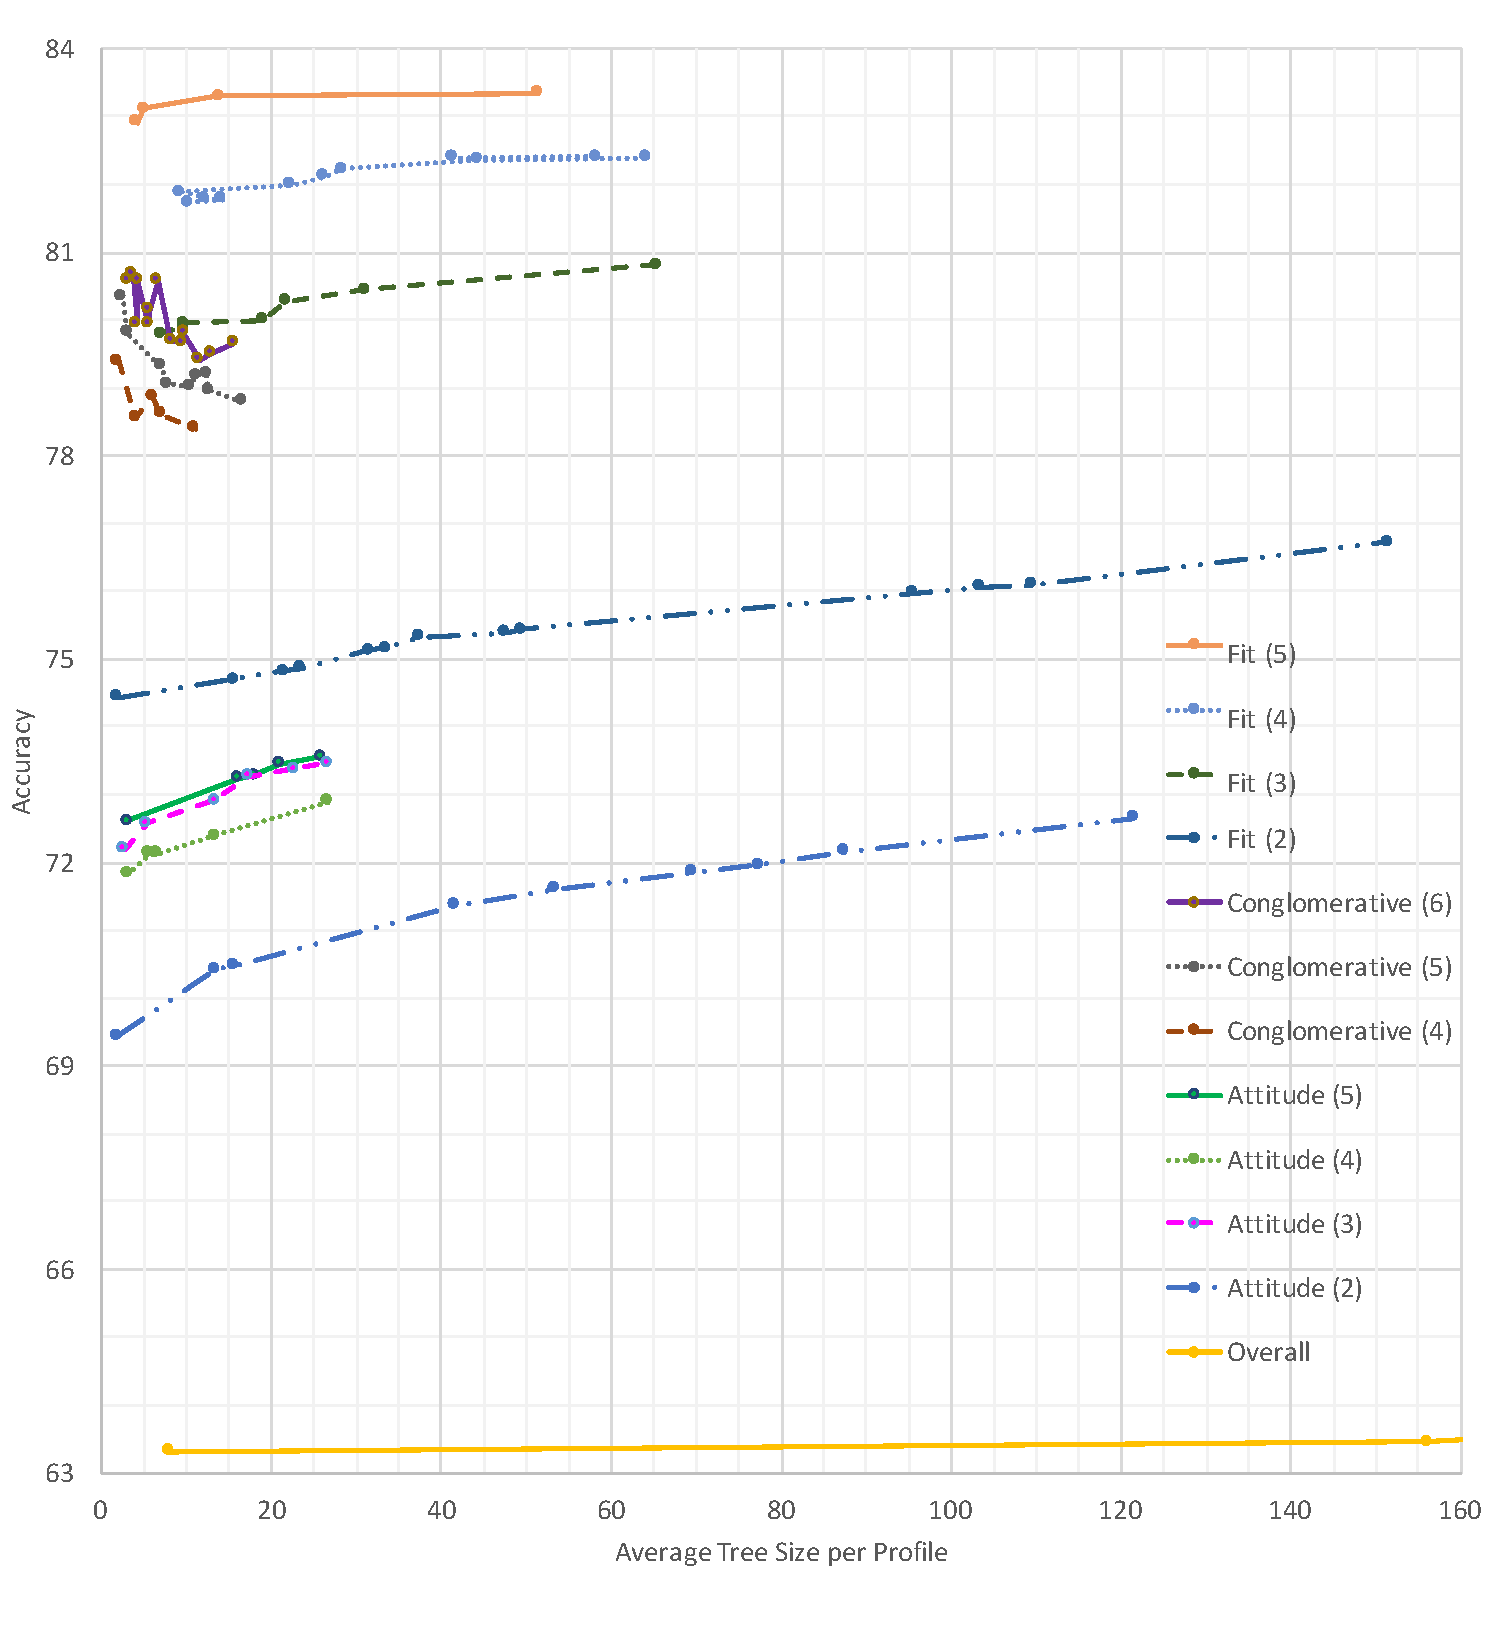
\includegraphics[width=0.7\textwidth]{figures/summaryAll.pdf}
	\caption{Summary of All our Approaches}
	\label{fig:summary}
\end{figure*}

The most parsimonious 2-profile fit-based solution (with an accuracy of 74.43\%) is the \emph{simplest} of all ``smart profile'' solutions: one profile is simply ``disable all'', while the other profile is the same as our OneR solution: ``disable sharing with third parties''. In fact, these profiles are so simple, that one might not even want to bother with presenting them to the user: in our current interface (see Figure~\ref{fig:interface2}) these defaults are incredibly easy for users to implement by themselves.

The same is true for the 4-profile agglomerative clustering solution (see Figure~\ref{fig:conglo_4_profile001}) and the 5-profile agglomerative clustering solution (see Figure~\ref{fig:conglo_5_profile001}): these profiles involve little more than a single high-level setting, which users can likely easily make by themselves. 

The 5-profile fit-based solution is the \emph{most accurate} of all ``smart profile'' solutions. The most parsimonious 5-profile fit-based clustering solution (Figure~\ref{fig:fit_5_profile001}) has an accuracy of 82.92\%. It has the following five profiles:
\begin{itemize}
	\item Enable all
	\item Enable local and remote storage, but disable third-party sharing
	\item Enable local storage only
	\item Enable local storage for everything except location-tracking, enable remote storage for everything except location- and presence-tracking, and disable third-party sharing
	\item Disable all
\end{itemize}
The fourth profile in this list specifies an interaction between between \textbf{Storage} and \textbf{Purpose}---something that is not possible in our current manual settings interface (which only allows interactions between \textbf{Who}, \textbf{What}, and \textbf{Purpose}). The next section will present a slightly altered interface that accommodates these profiles.

There is another 5-profile fit-based solution with a slightly higher accuracy (83.11\%) and a reasonably simple tree (5 nodes/profile on average). This solution is shown in Figure~\ref{fig:fit_5_profile003}. In this solution, the third profile (``enable local storage only'') is replaced by a slightly more complex profile (``enable local storage only, but not to recommend other services''). This profile specifies an additional interaction between \textbf{Storage} and \textbf{Action}. The next section will present a settings interface that accommodates this profile as well.

\begin{figure}
	\centering
	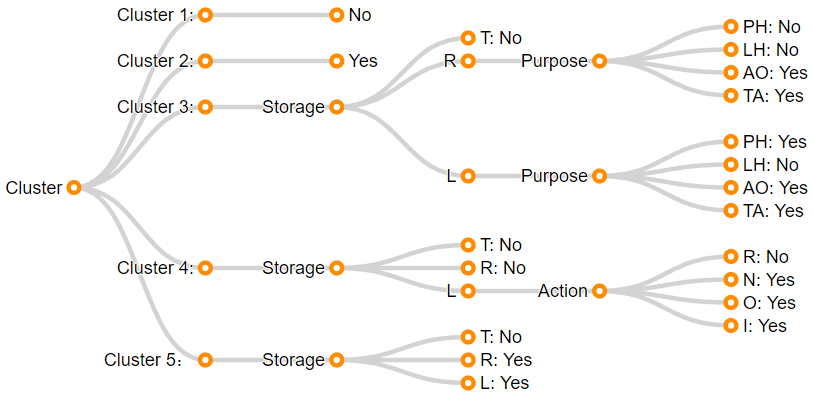
\includegraphics[width=0.6\textwidth]{figures/fit_5_profile003.png}
	\caption{A good 5-profile fit-based clustering solution (5 nodes/profile, Accuracy: 83.11\%). Parameter value abbreviations correspond to the ``code'' column in Table~\ref{tab:parameter2}.}
	\label{fig:fit_5_profile003}
\end{figure}

Other usable solutions are the 3-profile fit-based solution (Figure~\ref{fig:fit_3_profile001}) or the 4-profile fit-based solution (Figure~\ref{fig:fit_4_profile010}. However, like almost all of the less parsimonious solutions, these profiles involve higher-order interaction effects, e.g. between \textbf{Storage}, \textbf{Purpose}, and \textbf{Action}; and between \textbf{Storage}, \textbf{Purpose}, and \textbf{Who}. Consequently, a rather more complex interface is needed to accommodate these default profiles.

\section{Privacy-Setting Prototype Design Using Machine Learning Results (original work)}\label{sec:design_ml}
In Section~\ref{sec:design_stat} we developed a prototype interface that household IoT users can use to manually set their privacy settings (see Figure~\ref{fig:interface2}). Our machine learning analysis (Section~\ref{sec:predict}) resulted in a number of interesting solutions for ``smart profiles'' that would allow users of this interface to set their privacy settings with a single click (i.e., a choice of profile). While some of these profiles can be integrated in our prototype (e.g., the most parsimonious 2-profile fit-based solution and the 4-profile and 5-profile agglomerative solutions) other profiles have an interaction effect between variables that are modeled as independent in our current prototype interface (e.g., the two 5-profile fit-based solutions presented in Figures~\ref{fig:fit_5_profile001} and~\ref{fig:fit_5_profile003}).

In this section we therefore present two modified prototypes that are designed to be compatible with these two 5-profile solutions. These two solutions are not the most accurate, but they produce a parsimonious set of profiles that require only minimal alterations to our interface design. They thus provide the optimal trade-off between reduction accuracy, profile parsimony, and interface complexity.

\subsection{Interface for the 5-profile fit-based solution with an accuracy of 82.92\%}\label{sec:fit_simple}
This machine learning solution (Figure~\ref{fig:fit_5_profile001}) requires an interaction between the \emph{Storage} parameter and the \emph{Purpose} parameter---two parameters that are controlled independently in the prototype in Figure~\ref{fig:interface2}. Our solution is to slightly alter the interface, and add the profile selection page at the beginning of the interface (see Figure~\ref{fig:cluster_simple}): 
\begin{itemize}
	\item \textbf{Screen 1:} On this screen users choose their most applicable default profile. For some users, the selected profile accurately represents their preferences, while others may want to adjust the individual settings manually.
	\item \textbf{Screen 2:} After clicking `Next', users are given the option to select `Storage/Sharing  \& Device/Sensor Management' or `Data Use'.
	\item \textbf{Screen 3:} When users select either `Storage/Sharing \& Device/Sensor Management' they first get to set their sharing preferences for `local storage', `remote server' and `third party sharing' (\emph{Storage}). Each of these can independently be set to \emph{enabled} or \emph{disabled}, but users can also click on `More'. 
	\item \textbf{Screen 4:} When users select `More', they can manage \emph{Who-What-Purpose} combinations for that particular storage/sharing option.
	\item \textbf{Screen 5:} When users select `Data Use' on screen 2, they get to enable/disable the use of the collected data for various secondary purposes (\emph{Action}). 
\end{itemize}

\begin{figure*}
	\centering
	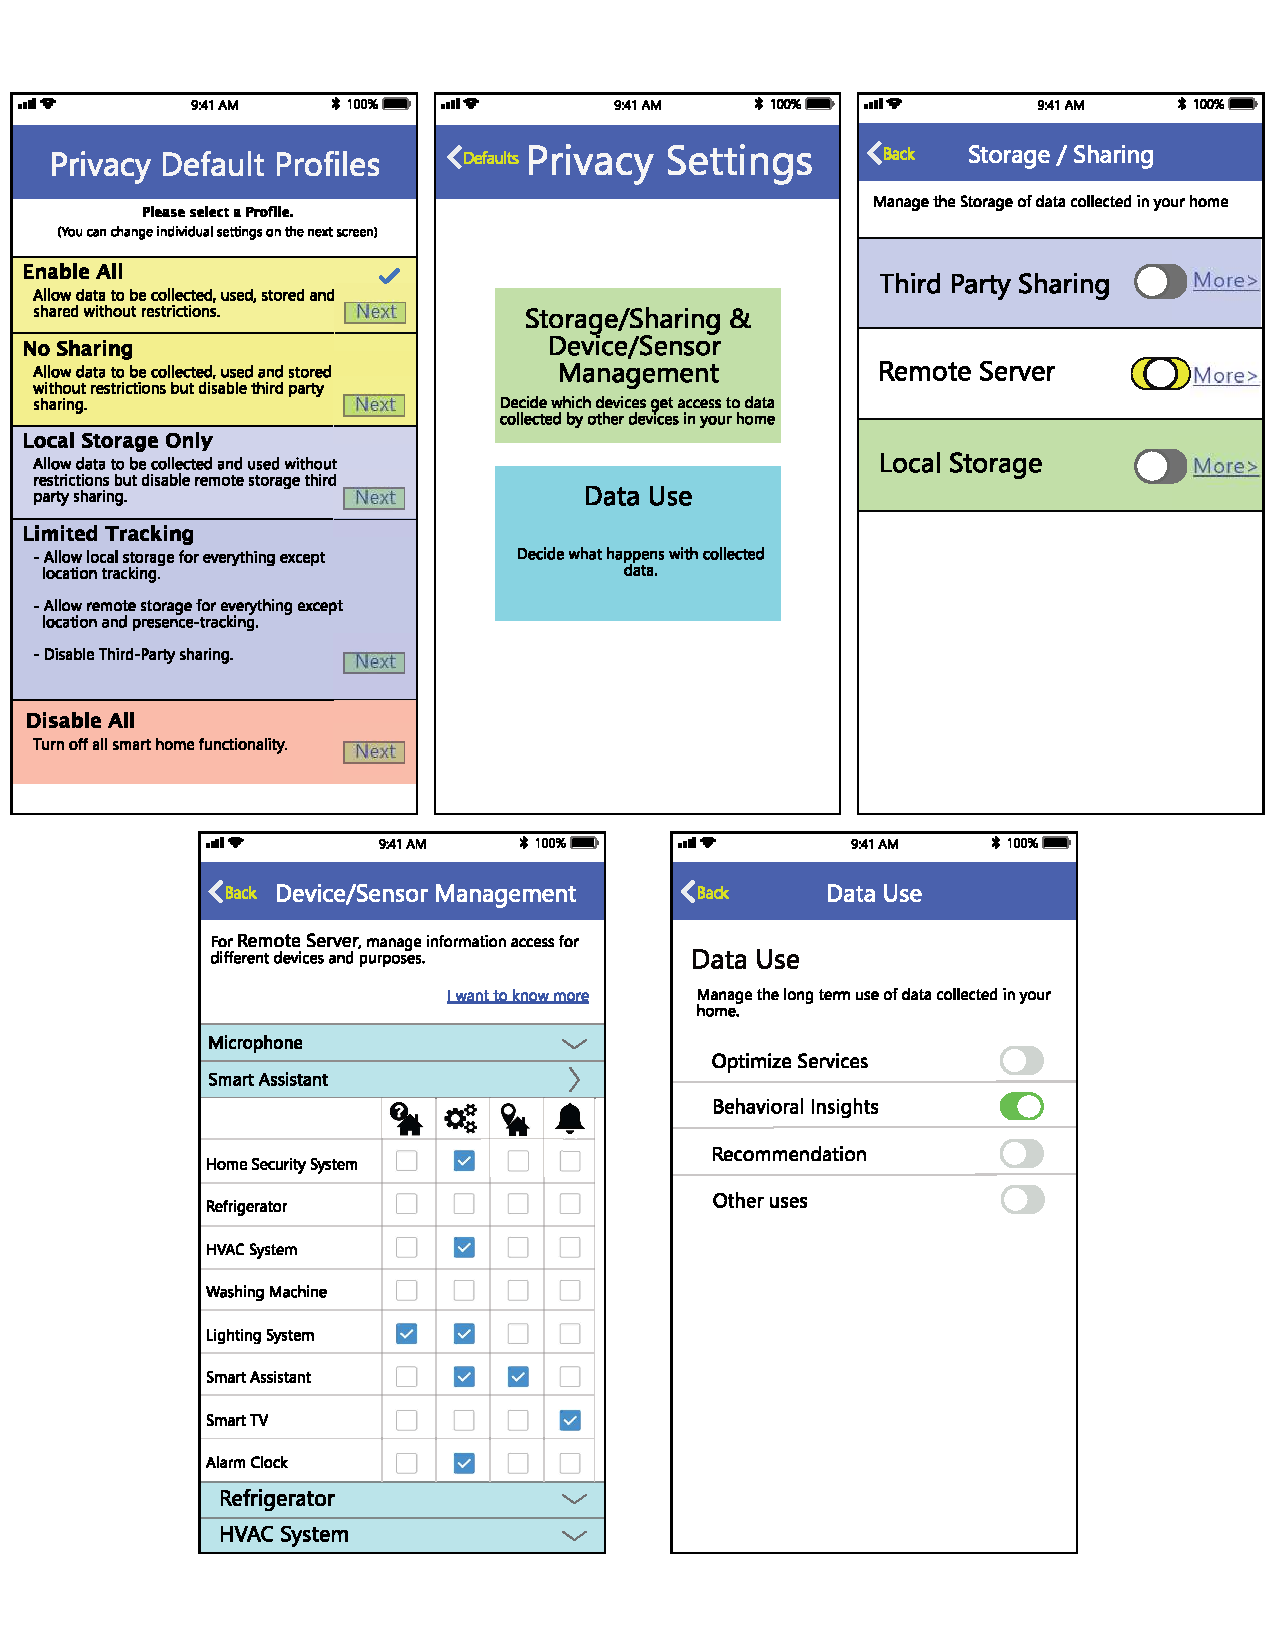
\includegraphics[width=0.8\textwidth]{figures/cluster_simple.pdf}
	\caption{Design for 5-Profile solution presented in Section~\ref{sec:fit_simple}. From top left, screen 1 is the profile selection page, screen 2 is the slightly altered landing page of our manual settings interface, screen 3 is the slightly altered Data Storage page, screen 4 (bottom left) is the Device/Sensor Management page, and screen 5 is the Data Use page.}
	\label{fig:cluster_simple}
\end{figure*}

\subsection{Interface for the 5-profile fit-based solution with an accuracy of 83.11\%}\label{sec:fit_complex}
The alternative machine learning solution presented in Figure~\ref{fig:fit_5_profile003} requires an additional interaction between the \emph{Storage} parameter and the \emph{Action} parameter. This requires us to slightly alter the interface again (see Figure~\ref{fig:cluster_complex}): 
\begin{itemize}
	\item \textbf{Screen 1:} The profile selection screen remains unchanged, with the exception that the `Local storage only' profile is replaced by the more complex `Local Storage \& No Recommendations' profile.
	\item \textbf{Screen 2:} After clicking `Next', users first get to set their sharing preferences for `local storage', `remote server' and `third party sharing' (\emph{Storage}). Each of these can independently be set to \emph{enabled} or \emph{disabled}, but users can also click on `More'.
	\item \textbf{Screen 3:} When users select `More', they are given the option to select either `Device/Sensor Management' or `Data Use'.
	\item \textbf{Screen 4:} When users select `Device/Sensor Management' they can manage \emph{Who-What-Purpose} combinations for that particular storage/sharing option.
	\item \textbf{Screen 5:} When users select `Data Use' they get to enable/disable the use of the collected data for various secondary purposes (\emph{Action}) for that particular storage/sharing option. 
\end{itemize}

\begin{figure*}
	\centering
	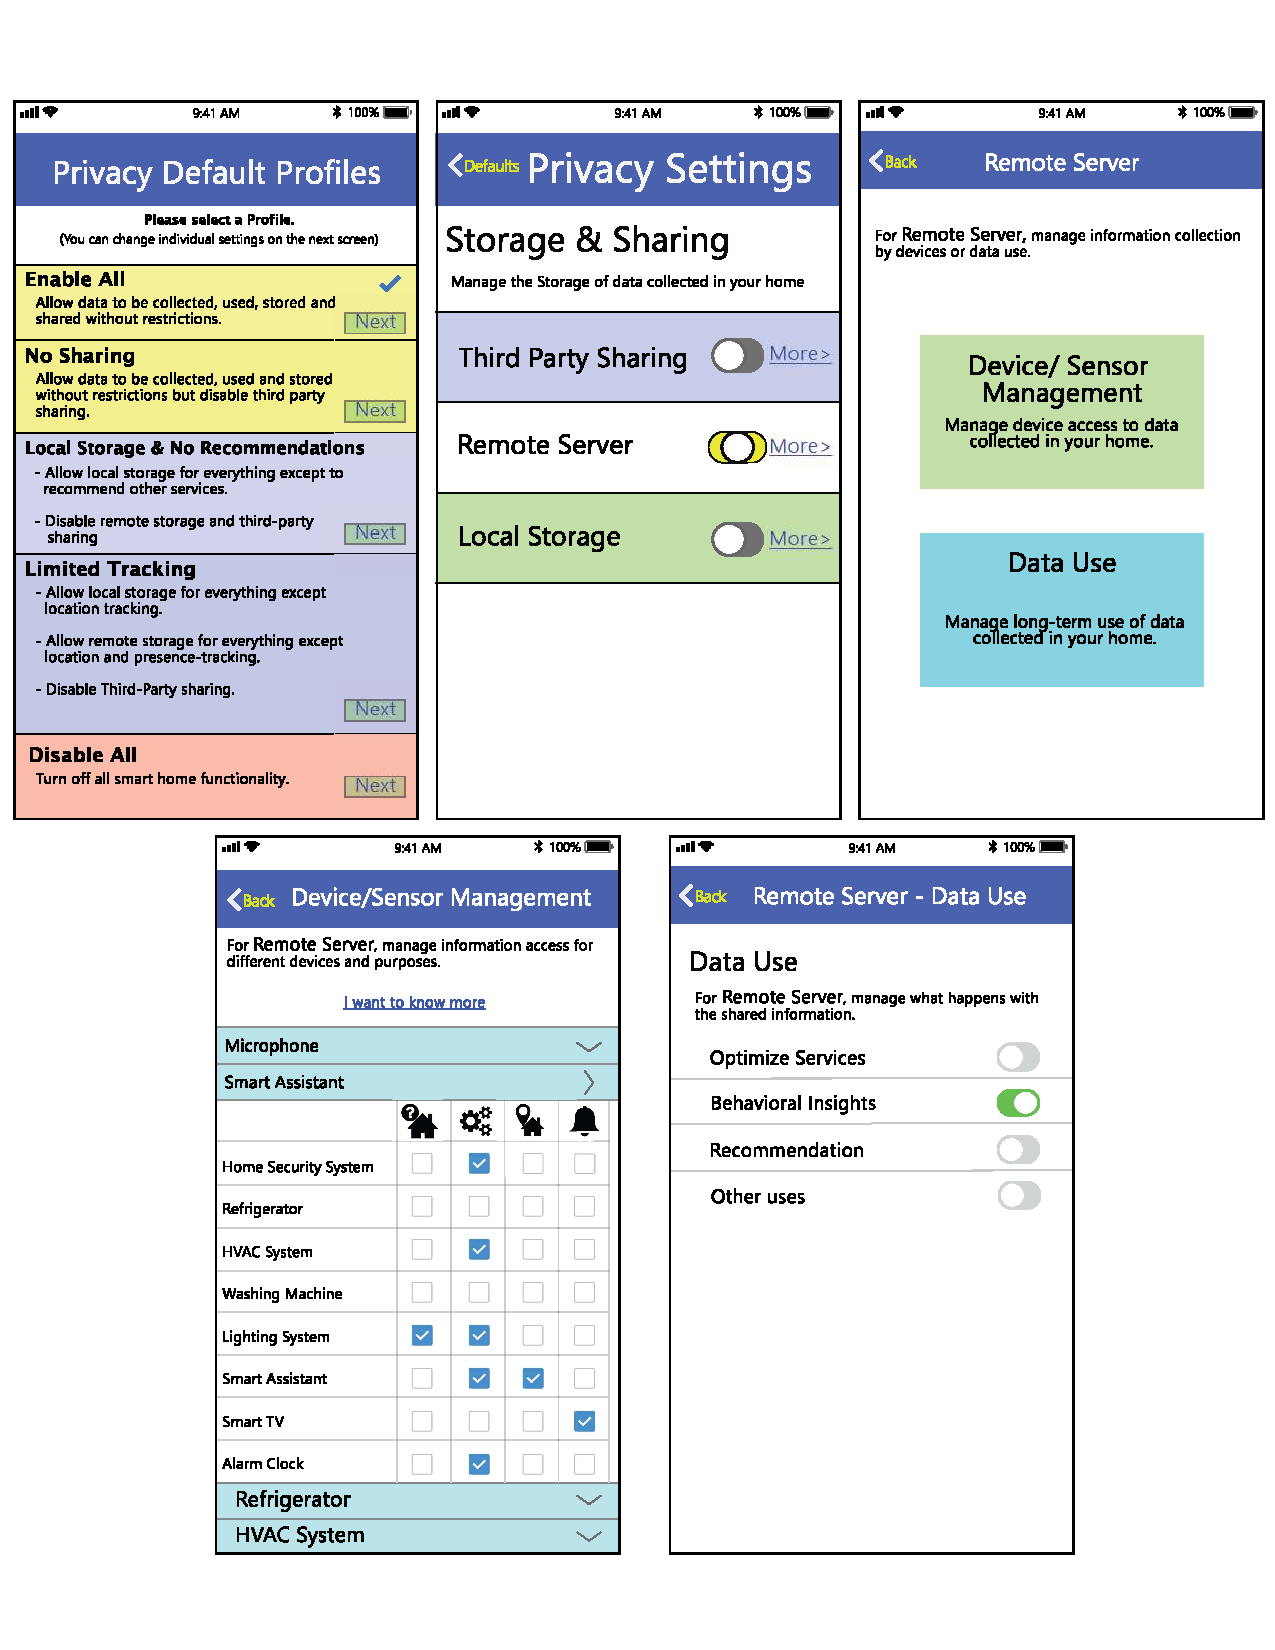
\includegraphics[width=0.8\textwidth]{figures/cluster_complex.pdf}
	\caption{Design for 5-Profile solution presented in Section~\ref{sec:fit_complex}. From top left, screen 1 is the profile selection page, screen 2 is the slightly altered Data Storage page, screen 3 follows the `More' button to offer access to screen 4 (bottom left, the Data Use page) and screen 5 (bottom right, the Device/Sensor Management page).}
	\label{fig:cluster_complex}
\end{figure*}

\subsection{Reflection on design complexity}
The interfaces presented in this section have an additional `layer' compared to the original interface presented in Section~\ref{sec:design_stat}. This additional layer makes setting the privacy settings manually more difficult, but it is necessary to accommodate the complexity of the smart profiles uncovered by our machine learning analysis. On the one hand, this demonstrates the value of developing a parsimonious machine learning model---the more accurate but more complex profiles that comprise some of the solutions in Section~\ref{sec:predict} are not only more difficult to explain to the user, they also contain more complex interactions between decision parameters, forcing the manual settings interface to become even more complex. A simple smart profile solution avoids such complexity in the interface. 

On the other hand, one should not over-simplify the profiles, lest they become overly generic and inaccurate in representing users' privacy preferences. Indeed, when we make our smart profile solutions more accurate, fewer users will need to make any manual adjustments at all, so we can allow some additional complexity in the interface.